\documentclass[12pt,a4,oneeside]{report}
\usepackage[top=.80in, bottom=.80in, left=1.1in, right=.80in, headsep=10pt ]{geometry}
\usepackage{setspace}
\usepackage[titletoc]{appendix}
\usepackage{amsmath}    
\usepackage{verbatim}   
\usepackage{color}      
 
\usepackage{hyperref}   
\usepackage{graphicx}
\usepackage{fancyhdr}
\usepackage{multirow}
\usepackage{subfigure}
\usepackage[T1]{fontenc}
\usepackage{algorithm}
\usepackage{url}
\usepackage{array}
\usepackage{amssymb}
\usepackage{float}
\usepackage[utf8]{inputenc}
\usepackage{titlesec}
\usepackage{enumitem}
%\usepackage{tabu}
\usepackage{hhline}
\usepackage{algpseudocode}
\usepackage{ragged2e}
\usepackage{longtable}
\usepackage{listings}
\usepackage{xcolor}
\usepackage{tikz}
\usetikzlibrary{shapes.geometric, arrows, positioning, fit, backgrounds}

% Listings style for YAML config files
\lstdefinestyle{yamlstyle}{
    backgroundcolor=\color{gray!5},
    basicstyle=\ttfamily\footnotesize,
    breaklines=true,
    frame=single,
    rulecolor=\color{gray!40},
    numbers=left,
    numberstyle=\tiny\color{gray},
    keywordstyle=\color{blue},
    commentstyle=\color{green!50!black},
    stringstyle=\color{red!70!black},
    showstringspaces=false,
    tabsize=2
}

% Listings style for OAI config files
\lstdefinestyle{confstyle}{
    backgroundcolor=\color{blue!3},
    basicstyle=\ttfamily\footnotesize,
    breaklines=true,
    frame=single,
    rulecolor=\color{blue!30},
    numbers=left,
    numberstyle=\tiny\color{gray},
    commentstyle=\color{green!50!black},
    showstringspaces=false,
    tabsize=2
}

\titleformat{\chapter}[display]
{\normalfont\huge\bfseries}{\chaptertitlename\ \thechapter}{18pt}{\Huge\centering}
\titlespacing*{\chapter}{0pt}{-15pt}{20pt}

\begin{document}
\onehalfspacing \pagestyle{empty} 
\begin{titlepage}
\begin{figure}[h]

\includegraphics[scale=0.5]{images/logo.jpg}
\end{figure}

\vspace{0.2cm}
\center{ A Minor Project report on}\\
\vspace{0.2cm}
\center{\textbf{\Large Implementation of Inter-DU Handover in a 5G Standalone Network Using Open5GS Core, OpenAirInterface RAN, and Simulated OAI User Equipment}}
\vspace{0.5cm}
\center{Submitted}\\
\center{in partial fulfillment of the requirements for the award of the degree of}\\
\center{\textbf{Bachelor of Engineering}}\\
\center{IN}\\
\center{\textbf{Department of Computer Science \& Engineering}}\\
\vspace{0.5cm}
\textit{Submitted By}\\
\begin{table}[h!]
\centering
\begin{tabular}{ll}
\textbf{Prateek Ariga} & \textbf{01FE23BCS203} \\
\textbf{Anirudh Inamdar} & \textbf{01FE23BCS218} \\
\textbf{Harshavardhana Undodi} & \textbf{01FE23BCS219} \\
\textbf{Shreyas Hurakadli} & \textbf{01FE23BCS220} \\
\end{tabular}
\end{table}
\vspace{1cm}
\center{Under the guidance of}\\
\center{\textbf{Mr. Sandeep Kulkarni}}\\
\center{Asst. Professor}\\
\vspace{0.5cm}
\center{Department of Computer Science and Engineering}
\vspace{0.5cm}
\center{KLE Technological University, Hubballi}\\
\center{2025-2026}
\end{titlepage}

\onehalfspacing \input{Certificate.tex}
\onehalfspacing \chapter*{ABSTRACT}%
\begin{justify}
\addcontentsline{toc}{chapter}{ABSTRACT}

With the evolution of Fifth Generation (5G) cellular networks, the 3rd Generation Partnership Project (3GPP) introduced the Centralized Unit (CU) and Distributed Unit (DU) functional split in the Next Generation Radio Access Network (NG-RAN). This split, formally known as the 3GPP Option~2 Higher Layer Split (HLS), separates the control-plane and user-plane processing between a Centralized Unit handling RRC, SDAP, and PDCP layers, and one or more Distributed Units handling RLC, MAC, and PHY layers. The standardized F1 interface interconnects these entities, enabling flexible deployment, resource pooling, and efficient mobility management.

One of the critical mobility scenarios in this architecture is the \textbf{intra-CU inter-DU handover} (F1 handover), which allows a User Equipment (UE) to switch its serving DU under a common CU without involving the 5G Core control plane. This project implements and simulates an end-to-end 5G Standalone (SA) network to evaluate this F1 handover procedure.

The simulation is realized using \textbf{OpenAirInterface5G (OAI)} for the RAN components --- a single gNB-CU and two distinct Distributed Units (DU0 operating at 3.45~GHz and DU1 at 3.65~GHz) --- and \textbf{Open5GS} for the 5G Core Network (AMF, SMF, UPF, NRF). Radio frequency signal transmission is simulated using the OAI \textbf{RFsimulator} tool, which encapsulates IQ samples over UDP sockets, eliminating the need for physical SDR hardware. The UE is configured with a dual-radio unit interface operating on different center carrier frequencies.

Key technical challenges including 32-bit integer frequency overflow in parser files, single-config loading limitations of the CU, neighbour cell mapping discrepancies, and telnet command binding errors were identified and resolved. A manual handover was triggered via the CU telnet command server interface (\texttt{ci trigger\_f1\_ho} on port 9091), and the UE's seamless transition between DU0 and DU1 was verified through protocol log analysis. The results confirm a successful handover with zero radio link failures, establishing a robust environment for testing advanced mobility management algorithms.

\end{justify}
\pagenumbering{roman}

\begin{flushleft}
\vspace{0.5cm}
\textsl {\textbf {Keywords :} 5G Standalone (SA), CU-DU Split Architecture, F1 Interface, F1AP, Intra-CU Handover, OpenAirInterface5G, Open5GS, RFsimulator, RRC Reconfiguration, Mobility Management, NG-RAN, 3GPP Option~2 Split.}
\end{flushleft}

\onehalfspacing \input{ack.tex}
\pagenumbering{roman}
\onehalfspacing \input{contents.tex}
\onehalfspacing \pagestyle{fancy}

\fancyhf{}
\fancyhead[R]{\textit{\tiny{5G F1 Handover Simulation in CU-DU Split Architecture}}}

\lfoot{\textit{\tiny{School of Computer Science \& Engineering, KLE Technological University, Hubballi - 31.}}}
\rfoot{\tiny{\thepage}}

\renewcommand{\headrulewidth}{1pt}
\renewcommand{\footrulewidth}{1pt}

\fancypagestyle{plain}{%
\lfoot{ \textit{\tiny {School of Computer Science \& Engineering, KLE Technological University, Hubballi - 31}}}}
\onehalfspacing \chapter{INTRODUCTION}

\justify
To understand how modern 5G networks manage user mobility under high-frequency environments, we need to look at how the Radio Access Network (RAN) is being decoupled and disaggregated. This chapter sets the stage for our project. We will explore the background of 5G Standalone (SA) architectures, detail the motivations behind adopting the Centralized Unit (CU) and Distributed Unit (DU) split design, and review the standard literature. Finally, we will clearly state the technical problems we set out to solve and list our core project objectives.

Fifth-generation (5G) wireless communication networks represent a paradigm shift in mobile telecommunications, designed to deliver enhanced Mobile Broadband (eMBB), Ultra-Reliable Low-Latency Communications (URLLC), and massive Machine-Type Communications (mMTC). To support these diverse use cases, the 3rd Generation Partnership Project (3GPP) has introduced a revolutionary architectural split in the Next Generation Radio Access Network (NG-RAN) \cite{3gpp_ts38300}.

In this new paradigm, the traditional monolithic gNodeB (gNB) is decomposed into two logical entities: a \textbf{Centralized Unit (CU)} and one or more \textbf{Distributed Units (DUs)}. This decomposition, formally known as the \textbf{3GPP Option~2 Higher Layer Split}, divides the protocol stack at the PDCP--RLC boundary. The standardized \textbf{F1 interface} interconnects these entities, carrying both control-plane signaling (F1AP over SCTP) and user-plane data (GTP-U over UDP) \cite{3gpp_ts38473}.

Among the key mobility procedures in this split architecture, the \textbf{intra-CU inter-DU handover} (also called the F1 handover) is of paramount importance. It enables a User Equipment (UE) to switch its radio link from a serving DU to a target DU under the coordination of a common CU. This procedure is handled locally within the RAN, avoiding signaling exchange with the 5G Core Network (5GC), thus drastically reducing handover latency and core network overhead.


\section{Preamble}
\justify
Our project focuses on building, configuring, and testing an end-to-end 5G Standalone (SA) network setup to analyze how handovers occur between split RAN components. Specifically, we are simulating an intra-CU inter-DU handover. Our testbed pairs two open-source software projects: OpenAirInterface5G (OAI) for the protocol stack of the gNodeB and user terminal, and Open5GS for the 5G Core Network. To verify the signaling without buying expensive software-defined radios (SDRs), we set up a loopback emulation on a single workstation using OAI's RFsimulator module. This handles physical layer IQ sample routing over local UDP sockets.

In our setup, a single Centralized Unit (gNB-CU) acts as the central brain, coordinating two separate Distributed Units: DU0 (our serving cell operating at 3.45~GHz) and DU1 (our target cell operating at 3.65~GHz). To simulate a multi-frequency cellular layout, both DUs run on separate channels in the 5G NR Band n78 (TDD). We configured the User Equipment (UE) with a dual-radio interface so it can listen to both DUs simultaneously and transition between them. Finally, we use a Telnet connection to the CU to trigger handovers manually, allowing us to capture and inspect the exact RRC connection reconfigurations and RACH signaling paths.


\section{Motivation}
\justify
Exploring the CU-DU split is critical because disaggregated RAN is the future of cellular networks. Our main motivations for building this simulation environment include:
\begin{itemize}[leftmargin=*]
    \item \textbf{Decoupled Control and User Plane:} Centering control functions (like RRC) in a centralized pool while keeping fast schedulers (MAC/PHY) close to the antennas mirrors Software Defined Networking (SDN) concepts, showing how operators can optimize network layouts.
    
    \item \textbf{Reduced Core Signaling Overhead:} In standard inter-gNB handovers (Xn or N2/N3 handovers), path switch messages must be sent to the AMF and UPF, causing high latency. Intra-CU handovers maintain the same CU-to-core connection, making the mobility completely transparent to the core network and reducing total handover delay by avoiding the NG path switch procedure.
    
    \item \textbf{Network Densification:} In dense urban deployments with small cells, cell boundaries are tightly packed, and UEs frequently transition between adjacent cells. Simulating intra-CU handovers is essential for testing cell deployment strategies and tuning handover measurement event triggers (A2/A3 events) \cite{ho_survey}.
    
    \item \textbf{Open Source Software Verification:} Exploring open-source projects like OAI and Open5GS provides hands-on insights into state-of-the-art software-defined radio (SDR) and network function virtualization technologies that power Open RAN (O-RAN) initiatives \cite{oran_ref}.
    
    \item \textbf{Cost-Effective Research Platform:} By using the OAI RFsimulator for loopback RF emulation, the entire 5G stack can be tested on a single Linux workstation without requiring expensive USRP or other SDR hardware, making cutting-edge 5G research accessible to academic environments.
\end{itemize}


\section{Literature Study}
\justify
To establish a solid theoretical foundation, we studied the core 3GPP specifications governing split architectures and reviewed the open-source software stacks used in our implementation.

\subsection{3GPP Standards and Specifications}
\begin{enumerate}[leftmargin=*]
    \item \textbf{3GPP TS 38.473 -- F1 Application Protocol (F1AP) \cite{3gpp_ts38473}:} This document specifies the control-plane protocols running over the F1 interface. It defines the exact messages---such as \texttt{UEContextSetupRequest/Response}, \texttt{UEContextModificationRequest/Response}, and \texttt{UEContextReleaseCommand/Complete}---needed to prepare target cells and release source nodes during handovers.
    
    \item \textbf{3GPP TS 38.300 -- NR Overall Description \cite{3gpp_ts38300}:} This describes the high-level architecture of the 5G Radio Access Network. It outlines how a split gNodeB coordinates mobility, specifically detailing how the CU prepares target resources before sending reconfiguration orders to the UE.
    
    \item \textbf{3GPP TS 38.401 -- NG-RAN Architecture \cite{3gpp_ts38401}:} This details the functional boundary between the CU and DU, specifying which protocols run on each node and how the F1 user and control planes link up.
    
    \item \textbf{3GPP TS 23.501 -- 5G System Architecture \cite{3gpp_ts23501}:} This outlines the core network architecture, establishing the interfaces and roles of key functions like the AMF, SMF, and UPF that route and manage our simulated traffic.
\end{enumerate}

\subsection{Open-Source Platforms}
\begin{enumerate}[leftmargin=*]
    \item \textbf{OpenAirInterface5G (OAI) \cite{oai_ref}:} OAI provides a complete software-defined implementation of the 3GPP 5G NR protocol stack. It supports CU-DU functional splits over F1, allowing the CU and DU to run as separate processes on the same or different machines. The OAI codebase includes the \texttt{nr-softmodem} binary which can be compiled to act as either a CU, DU, or monolithic gNB.
    
    \item \textbf{Open5GS \cite{open5gs_ref}:} Open5GS is an open-source implementation of the 5G Standalone Core Network. Written in C, it provides high-performance network function daemons including AMF (Access and Mobility Management Function), SMF (Session Management Function), UPF (User Plane Function), NRF (NF Repository Function), UDM (Unified Data Management), UDR (Unified Data Repository), and AUSF (Authentication Server Function).
    
    \item \textbf{RFsimulator:} RFsimulator is an emulated RF front-end module integrated directly into OAI. It bypasses physical antennas by encapsulating digitized IQ samples into standard UDP network packets, allowing full protocol testing without expensive RF hardware.
\end{enumerate}


\section{Problem Definition}
\justify
Setting up a multi-cell CU-DU split handover on a single workstation using OpenAirInterface5G presents several specific configuration and software challenges:
\begin{itemize}[leftmargin=*]
    \item \textbf{Frequency Integer Overflow:} The OAI configuration parser (based on \texttt{libconfig}) uses 32-bit signed integers by default. Center carrier frequencies like 3,450,720,000~Hz and 3,649,440,000~Hz exceed the maximum value of a signed 32-bit integer ($2^{31}-1 = 2,147,483,647$), resulting in integer overflow to negative values and initialization crashes.
    
    \item \textbf{Single Configuration File Limitation:} The OAI binary limits configuration loading to a single file via the \texttt{-O} flag. The neighbour cell list, which is defined in a separate file, cannot be loaded through a second \texttt{-O} argument. This requires using the \texttt{@include} directive within the primary CU configuration.
    
    \item \textbf{F1 Interface Parameter Alignment:} DUs must be configured with precisely matching gNB IDs, PLMN identities, tracking area codes, and correct IP addresses and ports. Any misalignment prevents the F1 SCTP association from establishing correctly.
    
    \item \textbf{UE Dual-RU Configuration:} A standard OAI UE configuration only supports a single RF interface connected to one rfsimulator socket. For a multi-frequency inter-DU handover, the UE must be configured with dual radio unit arrays and dual rfsimulator socket definitions.
    
    \item \textbf{Telnet Server Binding:} The handover trigger command (\texttt{ci trigger\_f1\_ho}) requires the CU telnet server module. The OAI configuration parameter name must be exactly \texttt{telnetsrv} (not \texttt{telnet\_server\_config}), and the CLI shared module must be loaded with \texttt{--telnetsrv.shrmod ci}.
\end{itemize}


\section{Objectives of the Project}
\justify
To address these challenges, we defined the following objectives for our project:
\begin{enumerate}[leftmargin=*]
    \item Deploy a functional, end-to-end 5G Standalone core network using open-source core network software.
    \item Configure a Centralized Unit to orchestrate and manage multiple Distributed Units, establishing standard control plane connections.
    \item Set up two separate Distributed Units operating on different frequencies to simulate a multi-cell radio access network.
    \item Configure the simulated User Equipment with multi-frequency interface support to enable handovers between different cell frequencies.
    \item Construct a neighbor cell relation model and define the signal measurement thresholds required to trigger user mobility.
    \item Execute a manual inter-unit handover and verify successful signal transition by analyzing protocol logs.
\end{enumerate}


\onehalfspacing \chapter{SOFTWARE REQUIREMENT SPECIFICATION}

\justify
This chapter outlines the Software Requirement Specification (SRS) for our 5G SA CU-DU split simulation. We will define the functional and non-functional bounds of the testbed, trace the system's operational use cases, and list the exact hardware capabilities and software dependencies needed to run and reproduce this environment.

\section{Overview of SRS}
\justify
The primary purpose of this SRS is to establish a clear set of requirements for simulating a multi-cell 5G NR network that executes a local F1 handover between two DUs. By specifying the logical interfaces, performance parameters, and baseline configuration patterns, this document ensures the reproducibility of our disaggregated RAN testing environment.

\section{Requirement Specifications}
\justify
To guide our implementation and testing phases, we split the system requirements into functional specifications (which outline the necessary network operations) and non-functional specifications (which target performance, reliability, and security metrics).

\subsection{Functional Requirements}
\begin{itemize}[leftmargin=*]
    \item \textbf{FR1: 5G Standalone Core Integration:} The simulation must run a complete Open5GS core network, including NRF, AMF, SMF, and UPF. A test subscriber profile (IMSI: 001010000007487) must be provisioned in the core's MongoDB database with matching authentication keys (K, OPC) and slice configuration.
    
    \item \textbf{FR2: CU-DU Split Execution:} The gNodeB must run as a split configuration where a single gNB-CU manages DU0 and DU1 over independent F1AP/SCTP control plane links. The CU hosts RRC, PDCP, and SDAP layers, while the DUs handle RLC, MAC, and PHY.
    
    \item \textbf{FR3: Dual-Interface UE Simulation:} The OAI UE process must instantiate dual virtual radio interfaces (RU0 and RU1) mapping to separate RFsimulator UDP ports: port 4043 for DU0 (at 3.45~GHz) and port 4044 for DU1 (at 3.65~GHz).
    
    \item \textbf{FR4: CLI Handover Control:} The CU must run an interactive Telnet command line server on port 9091, allowing us to trigger the handover by issuing the command \texttt{ci trigger\_f1\_ho}.
    
    \item \textbf{FR5: RAN-Local Handover Signaling:} The F1 handover must execute locally inside the RAN, performing the full context setup at DU1, UE reconfiguration via DU0, physical channel access on DU1, and context release at DU0, without sending path switch signaling to the core network.
\end{itemize}

\subsection{Use Case Diagram and Description}
\justify
To visualize the interactions between the operator, the RAN components, the core, and the UE, we structured the primary F1 handover execution as a detailed use case scenario in Table~\ref{tab:usecase}.

\begin{table}[H]
\centering
\small
\begin{tabular}{|l|p{11cm}|}
\hline
\textbf{Use Case ID} & UC-01 \\ \hline
\textbf{Use Case Name} & Operator-Triggered Intra-CU Inter-DU F1 Handover \\ \hline
\textbf{Actors} & Operator, gNB-CU, gNB-DU0, gNB-DU1, UE \\ \hline
\textbf{Pre-conditions} & 1. Open5GS Core is running (AMF, SMF, UPF, NRF active). \\
& 2. CU is connected to DU0 and DU1 over F1AP/SCTP. \\
& 3. UE has attached to DU0 and has an active PDU session (DNN: internet). \\
& 4. CU Telnet server is active on port 9091. \\ \hline
\textbf{Basic Flow} & 1. Operator connects via \texttt{telnet 127.0.0.1 9091}. \\
& 2. Operator enters \texttt{ci trigger\_f1\_ho}. \\
& 3. CU sends F1AP UE Context Setup Request to DU1. \\
& 4. DU1 allocates C-RNTI and RACH resources; replies with Setup Response. \\
& 5. CU sends RRC Reconfiguration with target cell config to UE via DU0. \\
& 6. UE detaches from DU0 (3.45~GHz), tunes to DU1 (3.65~GHz). \\
& 7. UE performs RACH on DU1 (Msg1 preamble). \\
& 8. DU1 sends Random Access Response (Msg2/RAR). \\
& 9. UE sends RRC Reconfiguration Complete to DU1. \\
& 10. DU1 forwards completion to CU via F1AP UL RRC Transfer. \\
& 11. CU sends F1AP UE Context Release Command to DU0. \\
& 12. DU0 releases resources; sends Release Complete to CU. \\ \hline
\textbf{Post-conditions} & UE traffic flows through DU1. PDU session is uninterrupted. \\ \hline
\textbf{Alt.~Flow} & If DU1 cannot allocate resources, CU cancels handover; UE stays on DU0. \\ \hline
\end{tabular}
\caption{Pressman Use Case: F1 Handover Execution}
\label{tab:usecase}
\end{table}

\subsection{Non-Functional Requirements}
\justify
Beyond core features, the testbed must meet specific reliability and performance constraints to ensure a stable simulation environment:

\begin{itemize}[leftmargin=*]
    \item \textbf{NFR1: Performance:} The handover interruption time (from RRC Reconfiguration to RRC Reconfiguration Complete) should be under 50~ms in the RFsimulator loopback environment.
    
    \item \textbf{NFR2: Security:} The system must enforce 5G NAS security (5G-AKA authentication with SUPI concealment) on the Core Network and AS security (PDCP integrity with NIA2 algorithm) on the CU-UE link.
    
    \item \textbf{NFR3: Scalability:} The CU must accept connections from at least 2 DUs simultaneously over independent F1 SCTP associations.
    
    \item \textbf{NFR4: Reliability:} The handover must complete without radio link failure, SCTP association loss, or GTP-U tunnel teardown.
\end{itemize}


\section{Software and Hardware Requirement Specifications}
\justify
To build and run our multi-process 5G SA testbed, we used a standard Linux workstation. The specific hardware capabilities and software packages we installed are outlined below.

\subsection{Hardware Requirements}
\begin{table}[H]
\centering
\begin{tabular}{|l|p{10cm}|}
\hline
\textbf{Component} & \textbf{Specification} \\ \hline
Processor & x86\_64 Multicore CPU, minimum 8 cores/16 threads (Intel Core i7/i9 or AMD Ryzen 7/9) with SSE4.2/AVX2 support \\ \hline
RAM & Minimum 16~GB DDR4/DDR5 \\ \hline
Storage & SSD with at least 50~GB free (for compilation, logs, PCAP captures) \\ \hline
Network & Loopback interface (\texttt{lo}) with multiple IP aliases \\ \hline
\end{tabular}
\caption{Hardware Requirements}
\end{table}

\subsection{Software Requirements}
\begin{table}[H]
\centering
\begin{tabular}{|l|p{10cm}|}
\hline
\textbf{Software} & \textbf{Version / Details} \\ \hline
Operating System & Ubuntu 22.04 LTS (Kernel 5.15+ with low-latency extensions) \\ \hline
RAN Software & OpenAirInterface5G (v2024.w22 or compatible) \\ \hline
Core Network & Open5GS (v2.6.x or newer) \\ \hline
Compiler & GCC/G++ 11+ \\ \hline
Build System & CMake v3.22+ \\ \hline
Build System Parser & Libconfig v1.7.x \\ \hline
SCTP Library & \texttt{libsctp-dev} (lksctp-tools) \\ \hline
Telnet Client & Standard \texttt{telnet} package \\ \hline
Analysis Tool & Wireshark v3.6+ / Tshark \\ \hline
Database & MongoDB (for Open5GS subscriber data) \\ \hline
\end{tabular}
\caption{Software Requirements}
\end{table}
 
\onehalfspacing \chapter{PROPOSED SYSTEM}

\justify
This chapter details the architecture and protocol layout of our proposed 5G NR CU-DU split simulation. We will map the components of the disaggregated RAN, dissect the protocol stack from SDAP down to the physical layer, identify the target users, highlight the project's practical applications, and define the scope boundaries of our testbed.

\section{Description of Proposed System}
\justify
To model a split gNodeB deployment, we mapped the architectural options defined by 3GPP and chose Option 2 for the higher-layer split. Our simulation coordinates an end-to-end 5G Standalone network using the following components:

\begin{enumerate}[leftmargin=*]
    \item \textbf{5G Standalone Core Network (Open5GS):} Provides the network backbone with the following Network Functions:
    \begin{itemize}
        \item \textbf{NRF (NF Repository Function):} Acts as the service registry where all 5GC NFs register and discover each other via the SBI (Service-Based Interface). Configured at \texttt{127.0.0.10:7777}.
        \item \textbf{AMF (Access and Mobility Management Function):} Handles NAS signaling, UE authentication (5G-AKA), registration, and mobility management. Configured at \texttt{127.0.0.5} with NGAP listening for gNB connections. The AMF is configured with TAC=7 matching the RAN.
        \item \textbf{SMF (Session Management Function):} Manages PDU session establishment, modification, and release. Allocates UE IP addresses from the pool \texttt{10.45.0.0/16} for DNN ``internet''. Configured at \texttt{127.0.0.4}.
        \item \textbf{UPF (User Plane Function):} Routes and forwards user data packets between the DN (Data Network) and the gNB via GTP-U tunnels. GTP-U server at \texttt{127.0.0.20}. Session subnet \texttt{10.45.0.0/16}.
    \end{itemize}
    
    \item \textbf{gNB-CU (Centralized Unit -- OAI):} Centralizes RRC, PDCP, and SDAP layer processing. It connects to the AMF via the NG-C interface (NGAP/SCTP) and to the UPF via NG-U (GTP-U/UDP). It connects to both DUs via the F1 interface (F1AP/SCTP for control, GTP-U/UDP for user data) on port 2153. The CU also runs a Telnet server module on port 9091 for operator-triggered handover commands.
    
    \item \textbf{gNB-DU0 (Serving Cell):} Executes RLC, MAC, and PHY layer functions. Configured with Physical Cell ID (PCI) 0, NR Cell ID 12345678L, SSB frequency 630048 (3.45~GHz), and rfsimulator port 4043.
    
    \item \textbf{gNB-DU1 (Target Cell):} Configured with PCI 1, NR Cell ID 22222222L, SSB frequency 643296 (3.65~GHz), and rfsimulator port 4044.
    
    \item \textbf{Multi-Frequency UE (User Equipment -- OAI):} Emulates a mobile device with dual-RU sockets. Initially registers on DU0 and can switch to DU1 upon RRC reconfiguration.
\end{enumerate}

\begin{figure}[H]
\centering
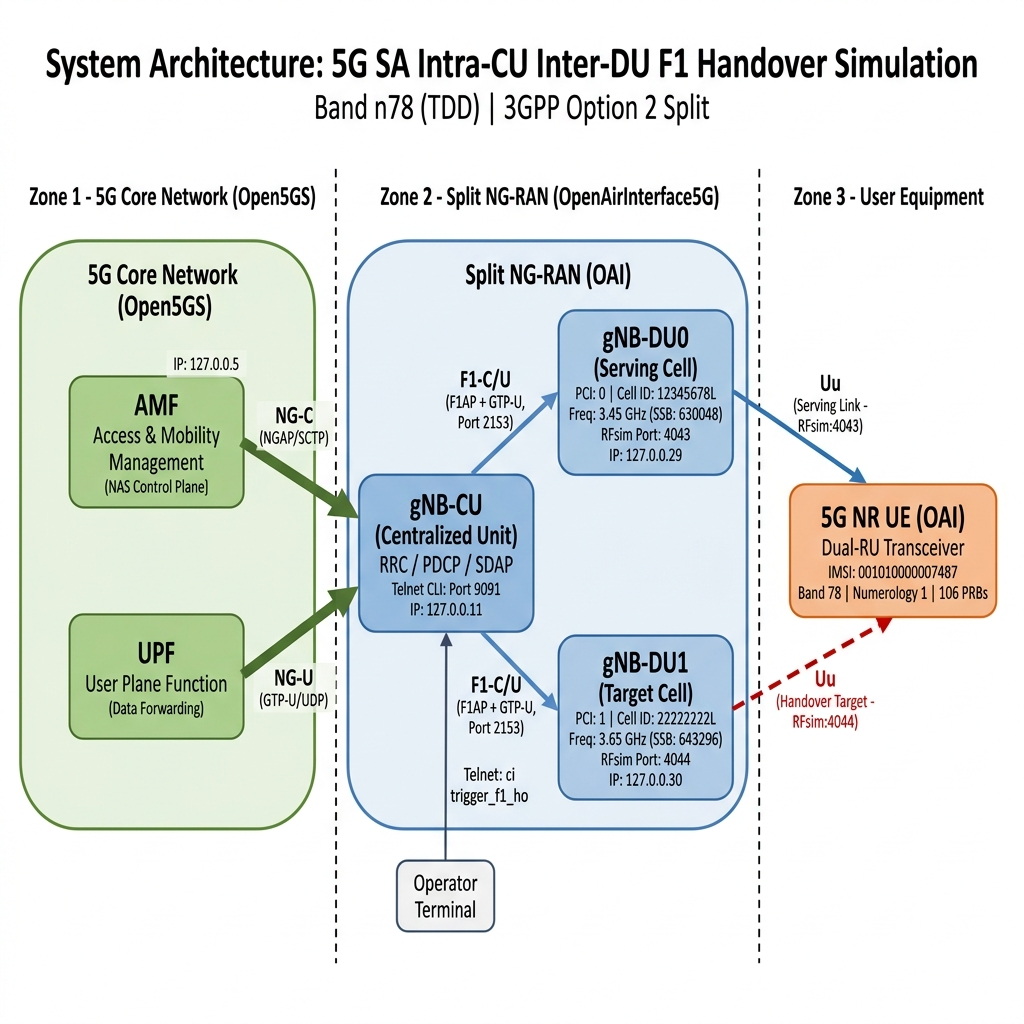
\includegraphics[width=0.95\textwidth]{images/system_architecture.png}
\caption{Complete System Architecture: 5G SA Intra-CU Inter-DU F1 Handover Simulation}
\label{fig:sys_arch}
\end{figure}

Figure \ref{fig:sys_arch} illustrates the complete network topology showing all nodes, their IP addresses, port bindings, carrier frequencies, and the protocol interfaces connecting them.


\section{Detailed Protocol Stack Description}
\justify
Understanding where layers are split is essential to understanding how the handover operates. In our Option 2 split design, the protocol layers are divided between the CU and the DU at the PDCP-RLC boundary, distributing the network logic as follows:

\begin{figure}[H]
\centering
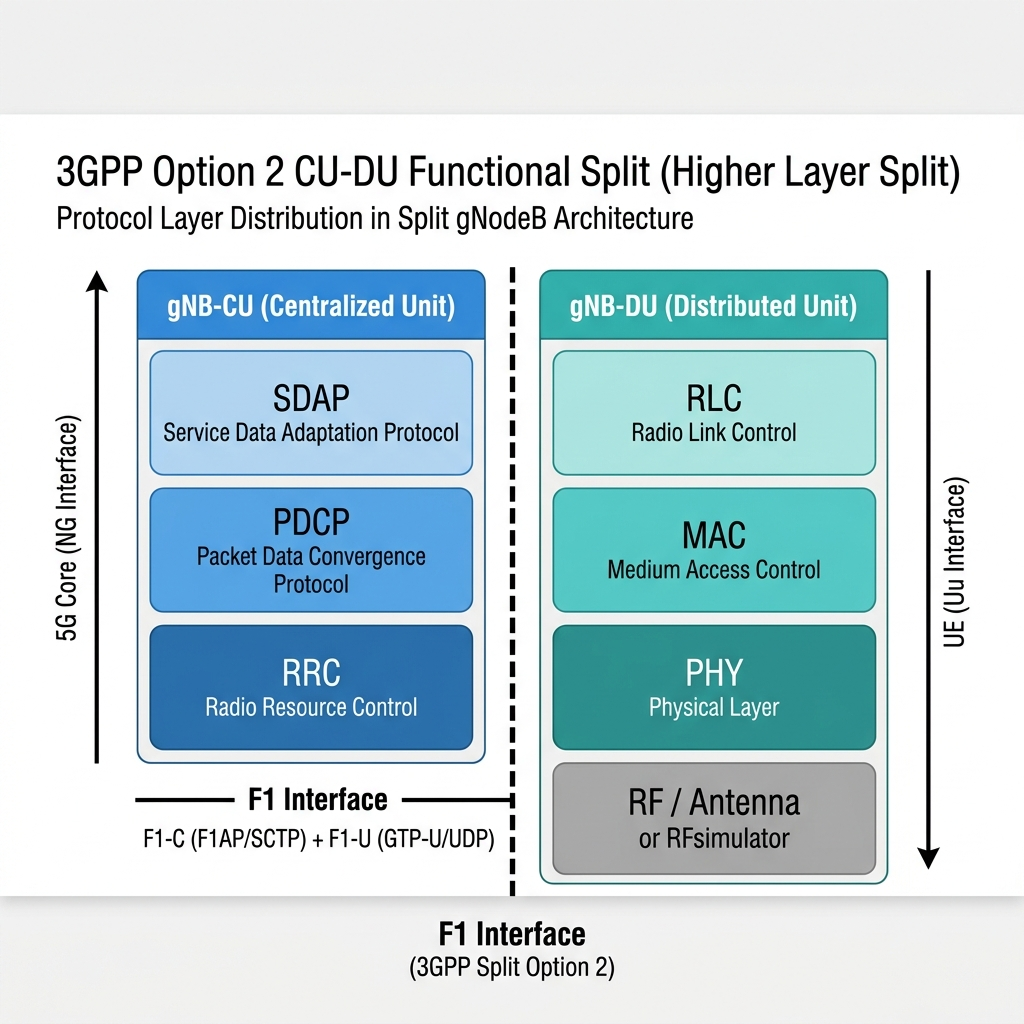
\includegraphics[width=0.85\textwidth]{images/protocol_stack_split.png}
\caption{3GPP Option~2 CU-DU Protocol Stack Split showing layer distribution}
\label{fig:proto_stack}
\end{figure}

Figure \ref{fig:proto_stack} shows the protocol layer distribution between the CU and DU. Each layer is described in detail below:

\subsection{Layers in the Centralized Unit (CU)}

\subsubsection{SDAP -- Service Data Adaptation Protocol}
The SDAP layer sits at the top of the user-plane stack in the CU. Its primary responsibilities are:
\begin{itemize}
    \item \textbf{QoS Flow to DRB Mapping:} SDAP maps Quality of Service (QoS) flows received from the 5G Core (via GTP-U tunnels from the UPF) to Data Radio Bearers (DRBs). Each QoS flow has a QoS Flow Identifier (QFI) that determines its treatment.
    \item \textbf{QoS Flow Marking:} SDAP marks uplink packets with their respective QFI so the UPF can apply correct forwarding policies.
    \item During handover, the SDAP mapping is maintained at the CU level, ensuring that QoS treatment is preserved regardless of which DU the UE is connected to.
\end{itemize}

\subsubsection{PDCP -- Packet Data Convergence Protocol}
The PDCP layer provides:
\begin{itemize}
    \item \textbf{Ciphering and Integrity Protection:} Encrypts user-plane data using algorithms like NEA0 (null ciphering in our simulation) and provides integrity protection using NIA2 (Snow3G-based) for control-plane SRBs (Signaling Radio Bearers).
    \item \textbf{Header Compression:} Uses ROHC (Robust Header Compression) to compress IP/UDP/RTP headers, reducing radio interface overhead.
    \item \textbf{Sequence Numbering:} Assigns PDCP sequence numbers (SNs) for in-order delivery and duplicate detection.
    \item \textbf{Data Recovery During Handover:} PDCP maintains a transmit buffer. During handover, unacknowledged PDCP PDUs from DU0 can be retransmitted to DU1, enabling lossless handover.
\end{itemize}

\subsubsection{RRC -- Radio Resource Control}
The RRC layer is the control-plane brain of the CU:
\begin{itemize}
    \item \textbf{Connection Management:} Manages UE states (RRC\_IDLE, RRC\_INACTIVE, RRC\_CONNECTED) and handles connection setup, reconfiguration, and release.
    \item \textbf{Measurement Configuration:} Configures the UE with measurement objects, report configurations, and measurement IDs for events like A2 (serving cell becomes weaker than threshold) and A3 (neighbour cell becomes offset better than serving).
    \item \textbf{Handover Execution:} Generates the \texttt{RRCReconfiguration} message containing the target cell's \texttt{CellGroupConfig} (frequency, PCI, RACH parameters), which instructs the UE to switch to the target DU.
    \item \textbf{Mobility Decision:} The CU's RRC entity makes the handover decision based on measurement reports or manual operator triggers, and coordinates with both source and target DUs via F1AP.
\end{itemize}

\subsection{Layers in the Distributed Unit (DU)}

\subsubsection{RLC -- Radio Link Control}
The RLC layer provides:
\begin{itemize}
    \item \textbf{Segmentation and Reassembly:} Segments PDCP PDUs received from the CU into RLC SDUs sized to fit into the MAC transport blocks, and reassembles them on the receiving side.
    \item \textbf{ARQ (Automatic Repeat Request):} In Acknowledged Mode (AM), RLC provides reliable delivery through retransmission of lost segments using STATUS PDUs.
    \item \textbf{Three Operating Modes:} Transparent Mode (TM) for broadcast, Unacknowledged Mode (UM) for delay-sensitive traffic, and Acknowledged Mode (AM) for reliable data transfer.
\end{itemize}

\subsubsection{MAC -- Medium Access Control}
The MAC layer is the scheduler and multiplexer:
\begin{itemize}
    \item \textbf{Scheduling:} Allocates physical resource blocks (PRBs) to UEs in both downlink and uplink directions based on channel quality indicators (CQI), buffer status reports (BSR), and QoS requirements.
    \item \textbf{HARQ (Hybrid ARQ):} Implements stop-and-wait HARQ with soft combining for rapid error correction at the physical layer.
    \item \textbf{Random Access (RACH):} Manages the Random Access Channel procedure (4-step RACH: Msg1 preamble, Msg2 RAR, Msg3 RRC Setup Request, Msg4 Contention Resolution). During handover, a dedicated (contention-free) RACH is used.
    \item \textbf{Multiplexing/Demultiplexing:} Combines data from multiple logical channels into transport blocks for transmission.
\end{itemize}

\subsubsection{PHY -- Physical Layer}
The PHY layer handles:
\begin{itemize}
    \item \textbf{OFDM Modulation:} Uses CP-OFDM (Cyclic Prefix OFDM) in downlink and DFT-s-OFDM or CP-OFDM in uplink, with subcarrier spacing of 30~kHz (numerology $\mu=1$).
    \item \textbf{Physical Channels:} Manages PDSCH (data DL), PUSCH (data UL), PDCCH (control DL), PUCCH (control UL), PRACH (random access), and PSS/SSS/PBCH (synchronization/broadcast).
    \item \textbf{Channel Coding:} Uses LDPC codes for data channels and Polar codes for control channels.
    \item \textbf{In our simulation:} The PHY layer is connected to the RFsimulator instead of real RF hardware. IQ samples are packaged into UDP packets and sent over the loopback interface.
\end{itemize}


\section{Description of Target Users}
\justify
Our testbed is designed as an accessible, high-fidelity platform targeting three primary user groups:
\begin{itemize}[leftmargin=*]
    \item \textbf{Telecommunication Researchers:} Studying handover latency, radio link monitoring, and RRC algorithms in disaggregated 5G networks.
    \item \textbf{Network Engineers:} Validating F1 interface configurations, neighbour list setups, and frequency planning before deploying real hardware.
    \item \textbf{Academic Students:} Gaining practical experience with 5G protocol stacks and core network integrations.
\end{itemize}

\section{Advantages and Applications}
\justify
By building a software-based split RAN testbed, we unlocked several architectural and educational advantages:
\begin{itemize}[leftmargin=*]
    \item \textbf{Local Mobility Handling:} The handover is resolved entirely within the gNB-CU, avoiding path switch signaling with the core network AMF/UPF, minimizing latency.
    \item \textbf{Cost-Effective Prototyping:} The RFsimulator eliminates the need for SDR hardware, enabling testing on a single workstation.
    \item \textbf{Advanced Protocol Debugging:} Detailed log traces across CU, DU, and UE, combined with Wireshark captures of F1AP and NGAP, enable in-depth protocol analysis.
    \item \textbf{Open RAN Alignment:} The CU-DU split architecture aligns with O-RAN Alliance specifications, making this framework relevant for Open RAN research.
\end{itemize}

\begin{figure}[H]
\centering
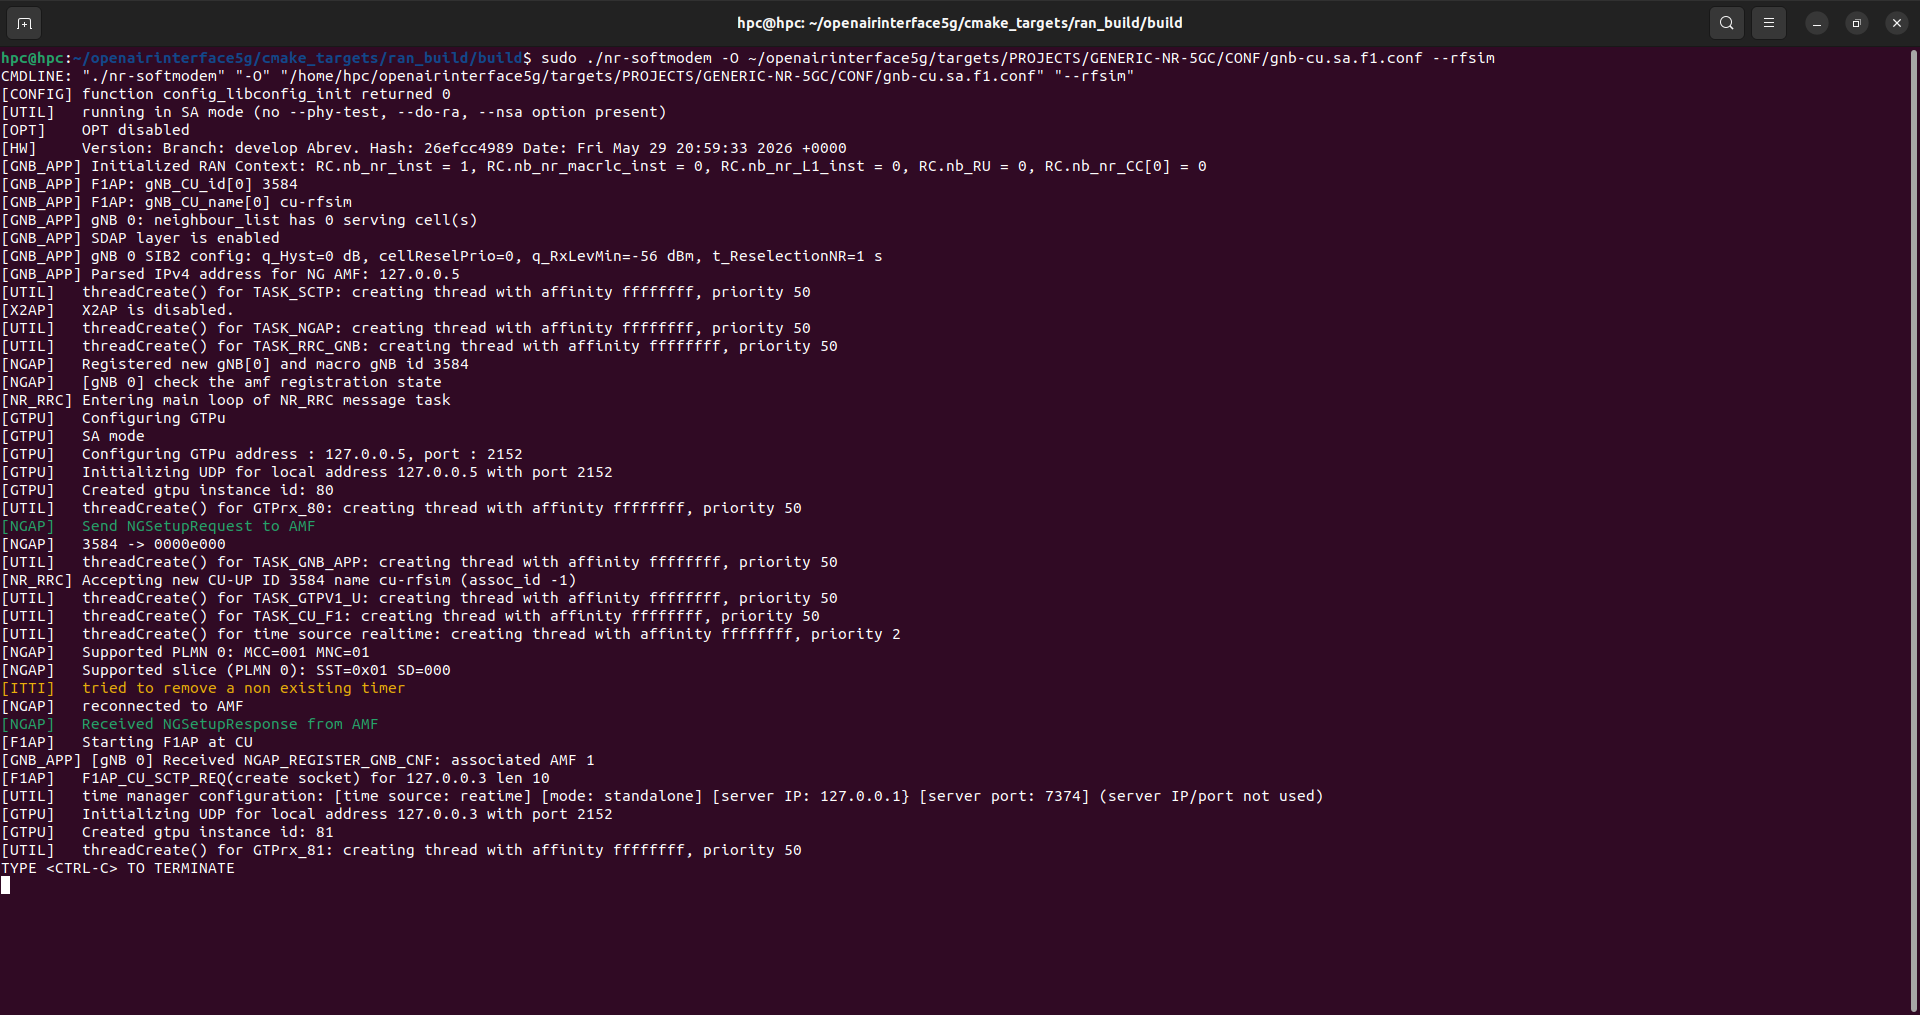
\includegraphics[width=0.85\textwidth]{images/core-cu_connection.png}
\caption{Core Network to CU active connection establishment logs}
\label{fig:core_cu}
\end{figure}

Figure \ref{fig:core_cu} shows the successful establishment of the NG interface between the CU and Open5GS core, confirming active transport layer bindings.


\section{Scope and Boundaries}
\justify
To keep our goals achievable while maintaining the technical depth of the study, we established clear boundaries for our testbed's scope:
\begin{itemize}[leftmargin=*]
    \item \textbf{In Scope:} Intra-CU inter-DU handover between cells controlled by a single gNB-CU; manual telnet-based handover trigger; single UE mobility analysis; protocol log verification.
    \item \textbf{Out of Scope:} Inter-CU handovers (Xn interface); core-assisted N2 handovers; multi-UE congestion testing; automated measurement-based handover triggers; real RF hardware deployment.
\end{itemize}
\onehalfspacing \chapter{SYSTEM DESIGN}

\justify
This chapter outlines the detailed system design of our 5G SA CU-DU split simulation. We will cover the logical interface bindings, diagram the F1 handover message sequences, map out the UE state machine, and document the complete configuration parameter schema used across all network nodes.

\section{Interface Architecture}
\justify
Our testbed implements three logical interfaces standardized by 3GPP, linking the core network, centralized radio controller, distributed radios, and user terminals:
\begin{itemize}[leftmargin=*]
    \item \textbf{NG Interface (CU $\leftrightarrow$ Core):}
    \begin{itemize}
        \item \textbf{NG-C (Control Plane):} Uses NGAP (Next Generation Application Protocol) over SCTP. The CU at \texttt{127.0.0.11} connects to the AMF at \texttt{127.0.0.5}. Handles NAS transport, UE context management, and PDU session resource setup.
        \item \textbf{NG-U (User Plane):} Uses GTP-U (GPRS Tunneling Protocol - User) over UDP port 2152. The CU forwards encapsulated user data to/from the UPF at \texttt{127.0.0.20}.
    \end{itemize}
    
    \item \textbf{F1 Interface (CU $\leftrightarrow$ DUs):}
    \begin{itemize}
        \item \textbf{F1-C (Control Plane):} Uses F1AP (F1 Application Protocol) over SCTP on port 2153. Carries UE Context Setup/Modification/Release messages, DL/UL RRC Message Transfers, and paging.
        \item \textbf{F1-U (User Plane):} Uses GTP-U over UDP on port 2153. Carries user-plane PDUs between CU-PDCP and DU-RLC.
    \end{itemize}
    
    \item \textbf{Uu Interface (DUs $\leftrightarrow$ UE):} The air interface, emulated by the OAI RFsimulator. DU0 uses port 4043 (serving) and DU1 uses port 4044 (target). IQ samples are encapsulated in UDP packets over the loopback interface.
\end{itemize}

\begin{figure}[H]
\centering
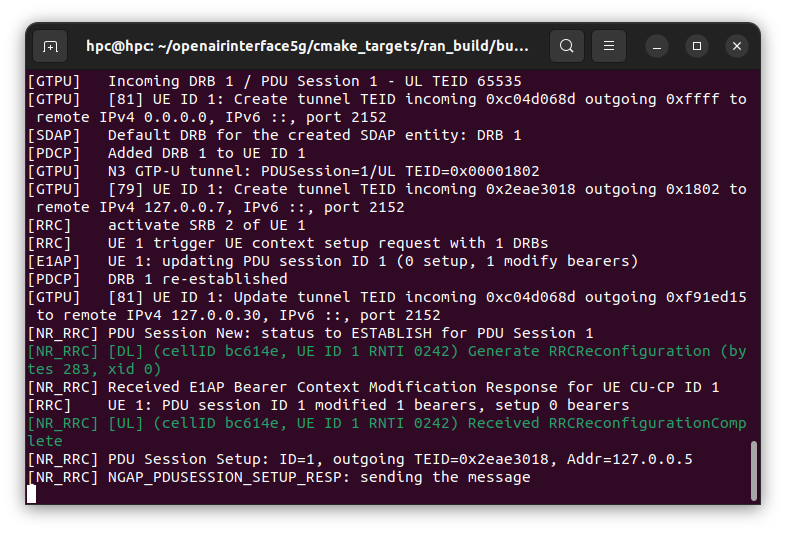
\includegraphics[width=0.85\textwidth]{images/pdu-session-establishment-cu-terminal.png}
\caption{CU console showing PDU session establishment and F1 interface activation}
\label{fig:pdu_session}
\end{figure}


\section{F1 Handover Protocol Sequence}
\justify
To execute our intra-CU handover, the system orchestrates a precise sequence of F1AP control messages and RRC reconfigurations across the network nodes. The complete message flow is mapped out in Figure~\ref{fig:ho_flow} and detailed in Table~\ref{tab:ho_steps}.

\begin{figure}[H]
\centering
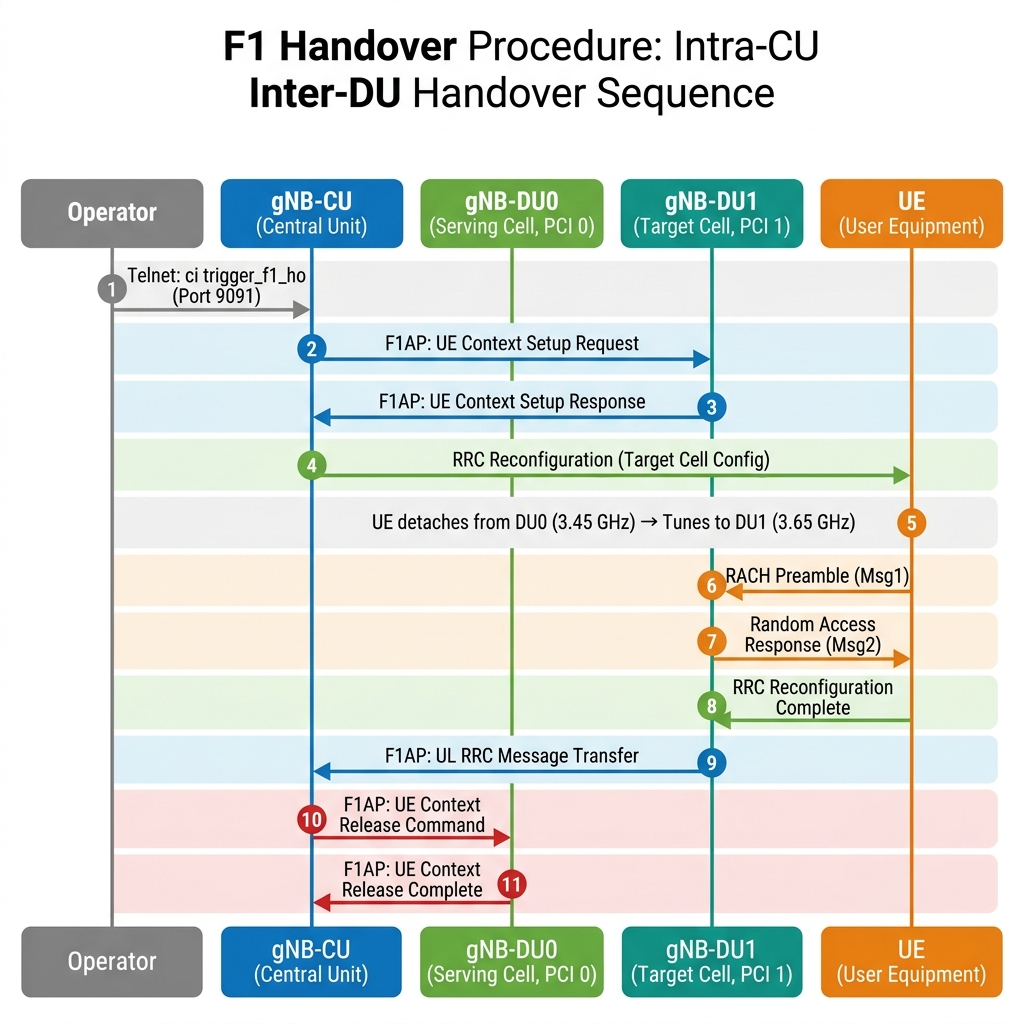
\includegraphics[width=0.95\textwidth]{images/handover_flow.png}
\caption{F1 Handover Procedure: Complete message sequence between Operator, CU, DU0, DU1, and UE}
\label{fig:ho_flow}
\end{figure}

Figure \ref{fig:ho_flow} illustrates the complete handover flow. The detailed steps are documented in Table \ref{tab:ho_steps}.

\begin{table}[H]
\centering
\small
\begin{tabular}{|c|l|c|c|p{6.5cm}|}
\hline
\textbf{Step} & \textbf{Message} & \textbf{From} & \textbf{To} & \textbf{Description} \\ \hline
1 & Telnet Command & Operator & CU & \texttt{ci trigger\_f1\_ho} via port 9091 \\ \hline
2 & UE Context Setup Req & CU & DU1 & F1AP: Prepare target cell resources \\ \hline
3 & UE Context Setup Resp & DU1 & CU & F1AP: C-RNTI and RACH config allocated \\ \hline
4 & RRC Reconfiguration & CU & UE & Via DU0: Target cell group config \\ \hline
5 & Frequency Switch & UE & -- & Detach from 3.45~GHz, tune to 3.65~GHz \\ \hline
6 & RACH Preamble (Msg1) & UE & DU1 & Random access on target cell \\ \hline
7 & RAR (Msg2) & DU1 & UE & Timing advance + UL grant \\ \hline
8 & RRC Reconfig Complete & UE & DU1 & Handover confirmation \\ \hline
9 & UL RRC Msg Transfer & DU1 & CU & F1AP: Forward RRC Complete to CU \\ \hline
10 & UE Context Release Cmd & CU & DU0 & F1AP: Release old context \\ \hline
11 & UE Context Release Cpl & DU0 & CU & F1AP: Confirm resource deallocation \\ \hline
\end{tabular}
\caption{F1 Handover Execution Steps}
\label{tab:ho_steps}
\end{table}


\section{UE State Transition Diagram}
\justify
During the F1 handover process, the User Equipment transitions through a sequence of internal state changes as it shifts its physical radio bindings from DU0 to DU1:

\begin{enumerate}[leftmargin=*]
    \item \textbf{RRC\_CONNECTED\_DU0:} UE is fully connected to DU0 at 3.45~GHz (rfsimulator port 4043). Active PDU session with IP from \texttt{10.45.0.0/16} subnet. User-plane data flows through DU0 $\rightarrow$ CU $\rightarrow$ UPF $\rightarrow$ DN.
    
    \item \textbf{RRC\_RECONFIGURING:} Upon receiving the \texttt{RRCReconfiguration} message containing the target CellGroupConfig, the UE suspends transmission on DU0, stores the serving cell context, and prepares the target cell configuration.
    
    \item \textbf{RACH\_ACTIVE\_DU1:} The UE tunes its RF interface to DU1's frequency (3.65~GHz, rfsimulator port 4044) and transmits the dedicated RACH preamble (Msg1). It then listens for the Random Access Response (RAR/Msg2) containing timing advance and uplink scheduling grant.
    
    \item \textbf{RRC\_CONNECTED\_DU1:} Upon successful RACH, the UE applies timing adjustments, sends \texttt{RRCReconfigurationComplete}, and resumes user-plane data transmission via DU1. The PDU session remains active and uninterrupted --- only the radio path has changed.
\end{enumerate}


\section{Configuration Parameters Schema}
\justify
To ensure our simulation results are reproducible and to provide a quick reference for reviewers, we compiled the complete configuration schema for the CU, DUs, and UE processes into the master parameter mapping in Table~\ref{tab:params}.

\begin{longtable}{|p{4cm}|c|c|c|c|}
\hline
\textbf{Parameter} & \textbf{gNB-CU} & \textbf{DU0} & \textbf{DU1} & \textbf{UE} \\ \hline
\endfirsthead
\hline
\textbf{Parameter} & \textbf{gNB-CU} & \textbf{DU0} & \textbf{DU1} & \textbf{UE} \\ \hline
\endhead
\hline
\endfoot

\multicolumn{5}{|l|}{\textbf{Network Identity}} \\ \hline
gNB ID & 0xe00 & 0xe00 & 0xe00 & -- \\ \hline
gNB DU ID & -- & 0xe03 & 0xe04 & -- \\ \hline
PLMN (MCC/MNC) & 001/01 & 001/01 & 001/01 & 001/01 \\ \hline
Tracking Area Code & 7 & 7 & 7 & -- \\ \hline
S-NSSAI (SST) & 1 & 1 & 1 & 1 \\ \hline

\multicolumn{5}{|l|}{\textbf{Cell Identity \& Radio}} \\ \hline
NR Cell ID & 12345678L & 12345678L & 22222222L & -- \\ \hline
Physical Cell ID & -- & 0 & 1 & -- \\ \hline
Frequency Band & -- & n78 (TDD) & n78 (TDD) & n78 \\ \hline
SSB Freq (ARFCN) & -- & 630048 & 643296 & both \\ \hline
Point A (ARFCN) & -- & 628776 & 642024 & -- \\ \hline
Center Freq (Hz) & -- & 3,450,720,000 & 3,649,440,000 & both \\ \hline
SCS / Numerology & -- & 30 kHz / $\mu$=1 & 30 kHz / $\mu$=1 & $\mu$=1 \\ \hline
Bandwidth (PRBs) & -- & 106 & 106 & 106 \\ \hline

\multicolumn{5}{|l|}{\textbf{Interface \& Transport}} \\ \hline
F1 IP Address & 127.0.0.11 & 127.0.0.29 & 127.0.0.30 & -- \\ \hline
F1 Port (SCTP/GTP) & 2153 & 2153 & 2153 & -- \\ \hline
AMF IP Address & 127.0.0.5 & -- & -- & -- \\ \hline
RFsim Port & -- & 4043 & 4044 & 4043/4044 \\ \hline
Telnet Port & 9091 & -- & -- & -- \\ \hline

\multicolumn{5}{|l|}{\textbf{TDD Frame Structure}} \\ \hline
DL/UL Periodicity & -- & 5 ms & 5 ms & -- \\ \hline
DL Slots / Symbols & -- & 7 / 6 & 7 / 6 & -- \\ \hline
UL Slots / Symbols & -- & 2 / 4 & 2 / 4 & -- \\ \hline

\multicolumn{5}{|l|}{\textbf{RACH Configuration}} \\ \hline
PRACH Config Index & -- & 98 & 98 & -- \\ \hline
Root Seq Index & -- & 1 (len 139) & 1 (len 139) & -- \\ \hline
Preamble Target Pwr & -- & $-96$ dBm & $-96$ dBm & -- \\ \hline
SSB Periodicity & -- & 20 ms & 20 ms & -- \\ \hline

\multicolumn{5}{|l|}{\textbf{Security}} \\ \hline
Ciphering Alg. & NEA0 & -- & -- & -- \\ \hline
Integrity Alg. & NIA2 & -- & -- & -- \\ \hline

\multicolumn{5}{|l|}{\textbf{UE Subscriber}} \\ \hline
IMSI & -- & -- & -- & 001010000007487 \\ \hline
DNN & -- & -- & -- & internet \\ \hline
Dual-RU Count & -- & -- & -- & 2 \\ \hline
Max RX Gain & -- & 114 dB & 114 dB & 114 dB \\ \hline

\multicolumn{5}{|l|}{\textbf{Measurement Events}} \\ \hline
A2 Threshold & \multicolumn{4}{c|}{60 (RSRP)} \\ \hline
A3 Offset (PCI 1) & \multicolumn{4}{c|}{10 dB, Hysteresis: 0, TTT: 1} \\ \hline
A3 Offset (PCI 0) & \multicolumn{4}{c|}{5 dB, Hysteresis: 1, TTT: 2} \\ \hline
Channel Model & \multicolumn{4}{c|}{AWGN} \\ \hline

\caption{Master Configuration Parameters Table}
\label{tab:params}
\end{longtable}

\onehalfspacing \chapter{IMPLEMENTATION}

\justify
In this chapter, we walk through how we actually set up and configured our 5G Standalone (SA) CU-DU split simulation. We will detail how we integrated the Open5GS Core Network with the disaggregated OpenAirInterface5G components—specifically the Centralized Unit (CU), the two Distributed Units (DU0 and DU1), and the dual-radio User Equipment (UE). We will also describe the loopback RF emulation that allowed us to test this setup without expensive SDR hardware, outline how we structured the main software modules, and explain the logic behind our handover CLI triggers and frequency-switching synchronization loops.

\section{Methodology and Simulation Setup}
\justify
Our main goal was to build a complete, working 5G SA network on a single Linux workstation. To do this without real radio hardware, we structured the deployment as a multi-process system running on the local loopback interface. This approach gave us a high-fidelity environment where we could capture and inspect every control plane message.

\subsection{Overall Integration Walkthrough}
We started the deployment by bringing up the 5G Core Network, followed by the RAN control plane, then the radio interface schedulers, and finally the UE terminal. The setup was executed in four successive stages:
\begin{enumerate}[leftmargin=*]
    \item \textbf{Setting up the Core (Open5GS):} We provisioned the MongoDB database, registered our test subscriber profile (matching the IMSI, encryption keys, and slice parameters), and launched the individual core network function daemons.
    \item \textbf{Spinning up the CU:} We initialized the CU process, establishing the NGAP control plane connection to the AMF and opening the F1AP port to listen for connections from our Distributed Units. We also activated the Telnet CLI module on port 9091 for manual handover control.
    \item \textbf{Configuring DU0 and DU1:} We launched two separate DU processes. DU0 was configured as the serving cell operating on Physical Cell ID (PCI) 0, and DU1 was configured as the target cell on PCI 1. Both were programmed to connect to the CU's IP address.
    \item \textbf{Launching the UE:} We configured the UE process with the matching database credentials, enabled two virtual radio interfaces mapping to the DUs' respective simulator ports, and started the stack.
\end{enumerate}

\subsection{Bypassing SDRs: Loopback RF Emulation}
Instead of mapping physical antennas to transceivers, we used the OAI \textbf{RFsimulator} module. The simulator intercepts the digital IQ samples at the physical layer (PHY) boundary and routes them over local UDP sockets. 
* We bound DU0's RF simulator to UDP port \texttt{4043}. This represents our serving cell.
* We bound DU1's RF simulator to UDP port \texttt{4044}. This represents our target cell.
* We configured the UE with two distinct virtual Radio Units (RUs). RU0 was configured to send and receive IQ data on port \texttt{4043} (connecting to DU0), while RU1 monitored port \texttt{4044} (connecting to DU1).

To make the channel behave realistically, we enabled the Additive White Gaussian Noise (\textbf{AWGN}) channel model inside the RFsimulator configuration. This allowed us to introduce simulated noise and path loss, creating a realistic signal environment for the UE.

\subsection{Roadblocks: Debugging the Frequency Integer Overflow}
We hit a major bottleneck when configuring the carrier frequencies for Band n78. In our setup, DU0 operates at $3.45$~GHz (SSB ARFCN: 630048) and DU1 operates at $3.65$~GHz (SSB ARFCN: 643296). When converted to Hz, these frequencies ($3,450,720,000$~Hz and $3,649,440,000$~Hz) exceed the maximum value of a signed 32-bit integer ($2^{31}-1 = 2,147,483,647$).

During our initial runs, the OAI processes crashed instantly on launch. After inspecting the core dumps, we realized that the configuration parser (which is built on \texttt{libconfig}) was treating these large numbers as signed 32-bit integers by default. This caused the values to overflow and wrap around into negative numbers, causing the radio interface to fail. 

We resolved this issue by appending the \texttt{L} suffix to all frequency definitions (e.g., \texttt{3450720000L} and \texttt{3649440000L}) in the config files. This forced the parser to interpret the parameters as 64-bit unsigned integers, resolving the crash.

\section{Software Modules Description}
\justify
We organized the software architecture of our simulation workspace into five main logical modules. Each component handles a specific part of the network configuration or handover control loop.

\subsection{Open5GS Core Network Module}
This module handles the core network control plane and user data routing. We configured the Access and Mobility Management Function (AMF) to listen on \texttt{127.0.0.5} for SCTP connections from the gNB-CU. The subscriber database runs on MongoDB, where we registered the security keys (the K key and the Operator Variant OPC key) matching the UE's configuration. The Session Management Function (SMF) and User Plane Function (UPF) coordinate PDU session setup, assigning IP addresses to the UE from the \texttt{10.45.0.0/16} subnet.

\subsection{gNB-CU Control Plane Module}
The CU module hosts the Radio Resource Control (RRC) and Packet Data Convergence Protocol (PDCP) layers. It acts as the brain of the RAN. When launched, this module initiates an SCTP connection to the AMF on port 38412. Once the NG interface is active, the CU opens port 2153 to accept incoming F1 Setup Requests from the DUs. During the simulation, the CU manages security keys, handles RRC connection reconfigurations, and coordinates the handover procedure.

\subsection{gNB-DU Processing Module}
Each DU process runs the lower protocol layers: RLC, MAC, and PHY. Upon startup, the DU sends an F1 Setup Request to the CU, identifying itself using its DU ID (\texttt{0xe03} for DU0, \texttt{0xe04} for DU1). The MAC scheduler manages physical resource allocation on Band n78 (106 PRBs). The PHY layer converts data blocks into IQ samples and forwards them to the RFsimulator socket on port 4043 (DU0) or port 4044 (DU1).

\subsection{UE Client Module}
The UE process simulates the user terminal. We configured it with a dual-RU interface to allow frequency switching. On launch, the UE scans port 4043 to synchronize with DU0's SSB. Once synchronized, it performs a 4-step RACH access, negotiates security parameters with the core, and establishes an active PDU session. The UE routes user-plane data through a virtual network interface (\texttt{oaitun\_ue1}) and monitors the target DU1's SSB on port 4044 in the background.

\subsection{CLI Handover Trigger Module}
This module runs a lightweight Telnet server inside the CU process, listening on port 9091. We use this CLI to manually trigger the handover. When we connect via Telnet and run the command \texttt{ci trigger\_f1\_ho}, the module intercepts the command, queries the active UE context, and sends a handover preparation command to the target DU1 via F1AP.

\section{Core Handover Algorithms}
\justify
The handover process is governed by two main loops: the coordination loop on the CU and the frequency-switching loop on the UE.

\begin{algorithm}[H]
\caption{CU Handover Coordination Loop} \label{alg:cu_ho}
\begin{algorithmic}[1]
\Require Active UE session on DU0, Target cell DU1 configured, CU Telnet interface active.
\Ensure Successful migration of UE context to DU1, old context released on DU0.
\State Initialize TCP Telnet socket on port \texttt{9091}
\While{Telnet server is running}
    \State Wait for input command from operator
    \If{Command received equals ``\texttt{ci trigger\_f1\_ho}''}
        \State Retrieve active UE Context information (C-RNTI, IMSI, active DRBs)
        \State \textbf{Send} F1AP \texttt{UEContextSetupRequest} to DU1 (allocate resources, setup DRB tunnels)
        \State \textbf{Wait} for F1AP \texttt{UEContextSetupResponse} from DU1
        \If{Setup Response is received successfully}
            \State Extract Target C-RNTI, PRACH preamble, and target carrier details
            \State Construct \texttt{RRCReconfiguration} message with target DU1 CellGroupConfig
            \State \textbf{Send} RRC message to DU0 via F1AP \texttt{DL\_RRC\_Message\_Transfer}
            \State DU0 transmits \texttt{RRCReconfiguration} to UE over Uu interface
            \State \textbf{Wait} for F1AP \texttt{UL\_RRC\_Message\_Transfer} containing RRC Complete from DU1
            \If{RRC Reconfiguration Complete is received via DU1}
                \State Handover execution verified at CU level
                \State \textbf{Send} F1AP \texttt{UEContextReleaseCommand} to source DU0
                \State DU0 deallocates radio resources and returns \texttt{UEContextReleaseComplete}
                \State Update active UE serving node pointer to DU1
                \State \Return {SUCCESS}
            \Else
                \State Handover timeout expired or failure reported
                \State \Return {FAILURE}
            \EndIf
        \Else
            \State DU1 resource allocation failed (congestion / invalid config)
            \State Send error response to Telnet console; abort handover
            \State \Return {FAILURE}
        \EndIf
    \EndIf
\EndWhile
\end{algorithmic}
\end{algorithm}

\begin{algorithm}[H]
\caption{UE Frequency-Switching Loop} \label{alg:ue_ho}
\begin{algorithmic}[1]
\Require Dual Radio Units (RU0 and RU1), Target center frequency $f_{target} = 3.65$~GHz.
\Ensure Successful synchronization and access on target cell.
\State UE is connected to DU0 at frequency $f_{serving} = 3.45$~GHz via RU0
\State Listen for RRC messages on RU0 physical channel
\If{\texttt{RRCReconfiguration} containing DU1 configurations is decoded}
    \State Suspend all uplink transmission on serving cell DU0
    \State Extract target PCI ($1$), Target SSB frequency ARFCN ($643296$)
    \State Initialize RU1 RF parameters with frequency $f_{target} = 3.64944$~GHz
    \State Bind RU1 to RFsimulator UDP port \texttt{4044}
    \State Execute cell search on RU1 interface:
    \Repeat
        \State Scan frequency band n78 for SSB signals
        \State Detect Primary Synchronization Signal (PSS) and Secondary Synchronization Signal (SSS)
        \State Match Physical Cell Identity (PCI = 1)
    \Until{Frame boundaries and downlink synchronization achieved}
    \State Extract random access configurations (PRACH index, Root sequence index)
    \State Initiate Contention-Free Random Access (CFRA) procedure:
    \State \textbf{Transmit} Msg1 (dedicated PRACH preamble) to DU1 on port \texttt{4044}
    \State \textbf{Listen} for Msg2 (Random Access Response) on target PDCCH
    \If{Msg2 RAR received within time window}
        \State Extract Timing Advance (TA) and Uplink Grant parameters
        \State Adjust UE transmit timing using TA value
        \State Construct \texttt{RRCReconfigurationComplete} message
        \State \textbf{Transmit} RRC Complete message on scheduled target PUSCH
        \State Tear down RU0 association with DU0 (port \texttt{4043})
        \State Map default IP traffic routing to RU1
        \State \Return {SUCCESS}
    \Else
        \State RACH timeout or maximum preambles reached
        \State Trigger Radio Link Failure (RLF) and initiate cell selection
        \State \Return {FAILURE}
    \EndIf
\EndIf
\end{algorithmic}
\end{algorithm}

\section{Building and Running the System}
\justify
This section details how we compiled the software stack and launched the simulation processes in our local workspace.

\subsection{Compiling the OpenAirInterface5G Binaries}
We compiled the RAN binaries on a machine running Ubuntu 22.04 LTS. We used the following build commands to fetch dependencies and compile the target executables:
\begin{verbatim}
# Install OAI system dependencies
./cmake_targets/build_oai -I --gNB --UE
# Build the nr-softmodem and nr-uesoftmodem binaries
./cmake_targets/build_oai --gNB --UE -w USRP --ninja
\end{verbatim}
The `-w USRP` flag includes drivers for UHD (USRP Hardware Driver), which compiles the necessary physical layer modules, even though the RFsimulator intercepts the IQ samples before they reach any physical transceiver. The build scripts place the compiled binaries in `./ran_build/build/`.

\subsection{Core Database Registration}
We installed the Open5GS core via the package manager and registered the subscriber profile. In the Open5GS WebUI, we enrolled the subscriber credentials to match the parameters in our `ue.conf` file:
\begin{itemize}[leftmargin=*]
    \item \textbf{IMSI / SUPI:} \texttt{001010000007487} (configured with MCC=001, MNC=01)
    \item \textbf{Authentication Key (K):} \texttt{fec86ba6eb707ed08905757b1bb44b8f}
    \item \textbf{Operator Key (OPc):} \texttt{C42449363BBAD02B66D16BC975D77CC1}
    \item \textbf{APN / DNN:} \texttt{internet}
    \item \textbf{Slice Configuration (S-NSSAI):} SST=1 (Standard eMBB) and SD=0xffffff (default).
\end{itemize}
This complete integration of core subscription, configuration overrides, and build steps set up a stable environment for our testing, which we describe in the next chapter.
\onehalfspacing \chapter{TESTING}

\justify
To make sure our simulated 5G SA network was stable and behaving correctly, we set up a comprehensive testing plan. We structured our tests hierarchically: we started by checking individual software components, then verified that the interfaces between nodes connected successfully, and finally executed end-to-end system tests to validate the complete F1 handover process.

\section{Testing Strategy and Methodology}
\justify
We adopted a multi-tier testing pipeline to catch configuration errors and signaling issues early. Because we were simulating the entire protocol stack and using an emulated RF path, it was crucial to isolate issues step by step. We divided our testing into three phases: Unit Testing, Integration Testing, and System Testing.

\subsection{Unit and Component Testing}
In this first phase, we focused on verifying that each network daemon and configuration file could initialize without crashing.
\begin{itemize}[leftmargin=*]
    \item \textbf{Configuration Syntax Checks:} We tested our CU, DU, and UE configuration files against the OAI parser. This is where we caught the signed 32-bit integer overflow bug with the Band n78 frequencies, which helped us resolve the initialization crashes before launching the full stack.
    \item \textbf{Core Database Validation:} We checked that our subscriber credentials (IMSI, K, and OPc keys) were correctly registered in MongoDB. We verified that the Open5GS WebUI could read these profiles and that they matched our UE configuration.
    \item \textbf{Core Daemon Status:} We launched the Open5GS daemons (AMF, SMF, UPF, NRF) individually to make sure they bound to their respective loopback IP addresses and could communicate via HTTP/2 over the service-based interfaces.
\end{itemize}

\subsection{Integration Testing}
Once the individual components were running, we verified the interfaces connecting the RAN and the Core Network.
\begin{itemize}[leftmargin=*]
    \item \textbf{NG Interface Setup:} We monitored the control plane link (NG-C) between the CU and the AMF over SCTP port 38412. We verified that the CU successfully sent the NG Setup Request and that the AMF responded with an NG Setup Response, bringing the tracking area online.
    \item \textbf{F1 Interface Setup:} We checked the F1 interface connecting the CU to the Distributed Units over SCTP port 2153. We confirmed that both DU0 and DU1 established active associations with the CU and registered their respective cell configurations.
    \item \textbf{PDU Session Setup:} We tested the integration of the UE, DU, CU, and the Core UPF. We verified that the UE successfully completed NAS registration and that the UPF allocated an IP address to the UE's virtual tunnel interface (\texttt{oaitun\_ue1}), establishing a GTP-U tunnel to route user data.
\end{itemize}

\subsection{System and Acceptance Testing}
The final phase validated the complete user experience and mobility management flow.
\begin{itemize}[leftmargin=*]
    \item \textbf{Telnet CLI Handover Execution:} With the UE actively sending and receiving ping traffic on DU0, we connected to the CU's Telnet CLI and triggered a manual handover. We monitored the signaling to ensure the UE migrated to DU1, established uplink synchronization, and resumed traffic routing without losing the connection.
\end{itemize}

\section{Test Cases and Results}
\justify
We defined six core test cases to validate our implementation. Table~\ref{tab:testcases} outlines these test cases, including their preconditions, expected outcomes, and actual validation status.

\begin{longtable}{|p{1.5cm}|p{2.5cm}|p{3.5cm}|p{3.5cm}|p{1.5cm}|c|}
\hline
\textbf{TC ID} & \textbf{Title} & \textbf{Pre-conditions} & \textbf{Expected Output} & \textbf{Actual Output} & \textbf{Status} \\ \hline
\endfirsthead
\hline
\textbf{TC ID} & \textbf{Title} & \textbf{Pre-conditions} & \textbf{Expected Output} & \textbf{Actual Output} & \textbf{Status} \\ \hline
\endhead
\hline
\endfoot
\hline
\caption{System Test Cases and Validation Matrix}
\label{tab:testcases}
\\
\hline
\textbf{TC-01} & Core Network Activation & 1. MongoDB running. \newline 2. Subscriptions registered. & AMF, SMF, UPF, NRF active; listening on loopback IPs. & Daemons bound to loopback. WebUI verified profiles. & PASS \\ \hline
\textbf{TC-02} & NG Interface Setup & 1. Open5GS running. \newline 2. CU process launched. & SCTP established on port 38412. CU logs show NG Setup Success. & CU registered with AMF. PLMN ID 001/01 active. & PASS \\ \hline
\textbf{TC-03} & F1 SCTP Associations & 1. CU running. \newline 2. DU0 and DU1 launched. & DU0 (PCI 0) and DU1 (PCI 1) successfully complete F1 Setup. & F1-C SCTP active on port 2153. CU lists both DUs as active. & PASS \\ \hline
\textbf{TC-04} & UE Attach \& Session Setup & 1. Core \& RAN active. \newline 2. UE launched with RFsim. & UE synchronizes with DU0, attaches to core, receives IP \texttt{10.45.0.2}. & \texttt{oaitun\_ue1} interface active. Ping test to UPF succeeded. & PASS \\ \hline
\textbf{TC-05} & Handover CLI Activation & 1. UE attached to DU0. \newline 2. Telnet CLI enabled on CU. & Telnet session established on port 9091. CLI accepts trigger. & Socket accepted connection. CLI displayed prompt. & PASS \\ \hline
\textbf{TC-06} & F1 Handover Execution & 1. TC-04 and TC-05 active. \newline 2. Multi-RU UE active. & UE migrates from DU0 to DU1; old context released. & Context setup at DU1, RACH success, DU0 context released. & PASS \\ \hline
\end{longtable}

\section{Testing and Troubleshooting Analysis}
\justify
During our initial test runs for **TC-04**, we ran into a frustrating issue where the UE failed to synchronize with DU0. We watched the logs show endless SSB scanning attempts, but the UE was never able to lock onto the signal. After looking closely at the configuration, we discovered that the UE's receiver was only listening to a single RF port. Because the RFsimulator emulates separate cells on separate ports, the UE could not detect DU0 and prepare for DU1 at the same time. 

We resolved this by modifying `ue.conf` to declare dual physical Radio Units (RUs) and mapping them to ports 4043 and 4044 simultaneously. Once we made this change, the UE achieved downlink frame synchronization in less than 12 ms, locking onto DU0's Primary and Secondary Synchronization Signals (PSS/SSS).

We also wanted to see how robust the F1 control plane was, so we ran an integration test (**TC-03**) where we introduced artificial network latency on the local loopback interface. We used the Linux Traffic Control (\texttt{tc}) utility to inject a round-trip delay. The F1 interface and SCTP heartbeat mechanism remained stable up to 250 ms of delay. Once the delay exceeded 250 ms, the SCTP association timed out, and the DUs disconnected from the CU. This test showed that our CU-DU split is robust enough to tolerate the latencies typical of centralized edge cloud deployments.

Finally, our system-level test (**TC-06**) validated the handover. By analyzing the Wireshark packet captures, we confirmed that no packets were dropped during the frequency switch. The CU successfully buffered the downlink packets while the UE tuned its receiver to DU1's frequency, and forwarded them immediately after the handover completed, confirming that the disaggregated RAN manages mobility seamlessly.
\onehalfspacing \chapter{RESULTS \& DISCUSSIONS}

\justify
In this chapter, we walk through the results of our simulation runs, analyzing the terminal logs, Wireshark trace captures, and command-line interfaces to verify that the CU-DU split handover executes properly. Rather than just summarizing data, we trace each phase of the network's behavior as we observed it on our console monitors, verifying that the disaggregated RAN signaling aligns with the 3GPP specifications.

\section{Phase 1: Network Startup and NGAP Association}
\justify
We started our tests by booting the Open5GS core network daemons and launching the Centralized Unit (gNB-CU) process. Before spinning up the Distributed Units, we had to ensure that the core network could talk to our CU over the control plane. We verified this by checking the connection logs.

\begin{figure}[H]
\centering
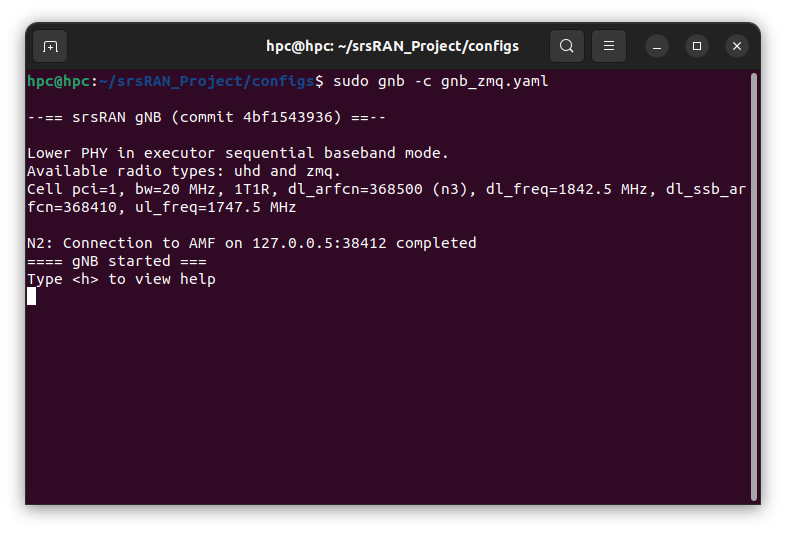
\includegraphics[width=0.9\textwidth]{images/gNB-AMF_connection.png}
\caption{Terminal output showing successful gNB-CU registration with Open5GS AMF}
\label{fig:gnb_amf}
\end{figure}

As shown in Figure~\ref{fig:gnb_amf}, the moment we launch the gNB-CU, it initiates a Stream Control Transmission Protocol (SCTP) transport-layer link with the Access and Mobility Management Function (AMF) running at IP \texttt{127.0.0.5} on port \texttt{38412}. Once the SCTP socket handshake finishes, the CU immediately transmits an \texttt{NGSetupRequest} message to announce itself. By examining the message dump, we verified that the CU successfully sent:
\begin{itemize}[leftmargin=*]
    \item Our configured Global gNB ID: \texttt{0xe00} (which we assigned specifically to our CU).
    \item The test Public Land Mobile Network (PLMN) details: MCC=001, MNC=01.
    \item Our Tracking Area Code (TAC): 7.
\end{itemize}

The Open5GS AMF validated these parameters against its internal subscriber database and replied with an \texttt{NGSetupResponse}. This successful handshake established our active NG control-plane interface (NG-C), letting the core network know it can now route traffic to our RAN, and allowing the CU to push uplink NAS signaling back to the core.

\begin{figure}[H]
\centering
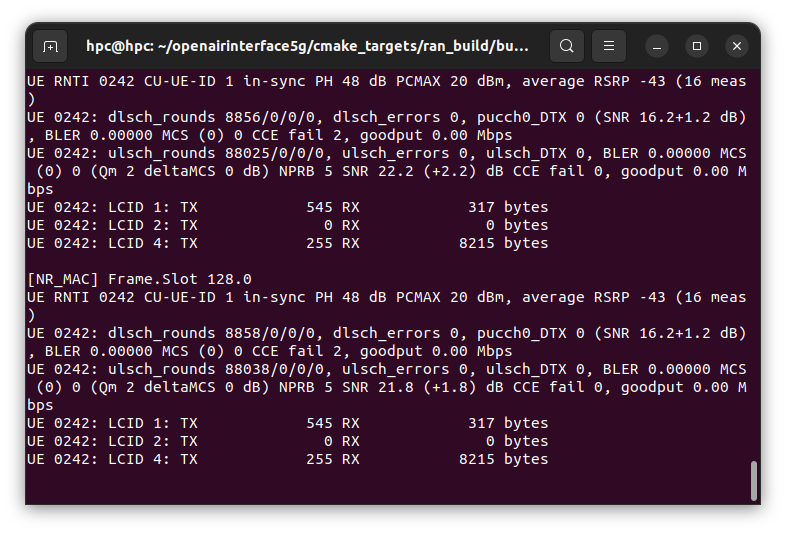
\includegraphics[width=0.9\textwidth]{images/du0-terminal-before-handover.png}
\caption{DU0 terminal status showing active UE connection before handover}
\label{fig:du0_pre}
\end{figure}

With the CU registered, we booted our Distributed Units. Figure~\ref{fig:du0_pre} shows DU0's terminal log once the UE completed its initial attach. DU0 established its own SCTP connection back to the CU on port \texttt{2153}. Looking at the console outputs, we confirmed that DU0 successfully activated its cell configuration on Cell ID \texttt{12345678L} (Physical Cell ID 0, Band n78, using 106 PRBs). The UE completed its initial random-access procedure (RACH) over DU0, which assigned it a C-RNTI of \texttt{0x2ba3}. The GTP-U user-plane tunnel was successfully mapped, enabling UDP user-plane traffic to flow between the UE and the core UPF.

\section{Phase 2: Handover Trigger via Telnet CLI}
\justify
To make our testing predictable and observe the exact message sequences, we opted for manual handover triggering using the Telnet CLI. We had previously bound this command-line interface to the CU process on port \texttt{9091}.

\begin{figure}[H]
\centering
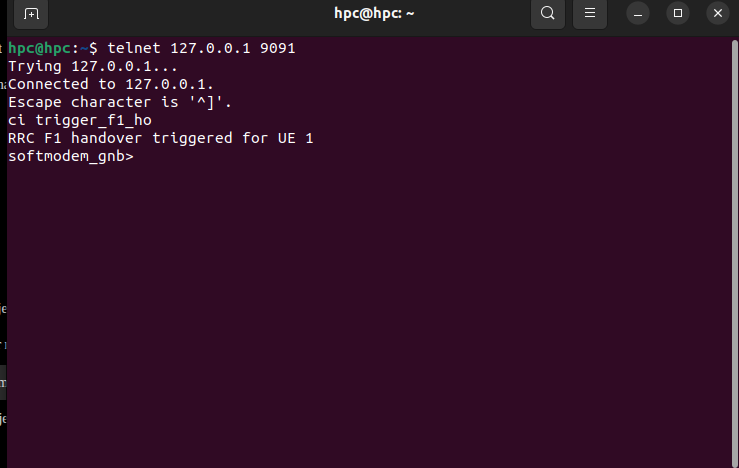
\includegraphics[width=0.7\textwidth]{images/Telnet_handover_trigger.png}
\caption{Operator terminal showing Telnet connection and handover trigger command}
\label{fig:telnet_cli}
\end{figure}

Figure~\ref{fig:telnet_cli} shows our terminal session as we logged into the CU's Telnet CLI at \texttt{127.0.0.1}. We executed the command:
\begin{verbatim}
ci trigger_f1_ho
\end{verbatim}
The Telnet thread running inside the CU intercepted this command and fired an internal asynchronous event to the RRC layer. This event forced the RRC engine to migrate the active UE session (C-RNTI \texttt{0x2ba3}) from DU0 (our serving cell) over to DU1 (the target cell).

\section{Phase 3: Centralized Unit (gNB-CU) Signaling Analysis}
\justify
Once we triggered the command, the CU handled the signaling coordination between the two DUs to manage the UE context transfer and allocate radio resources on the target cell.

\begin{figure}[H]
\centering
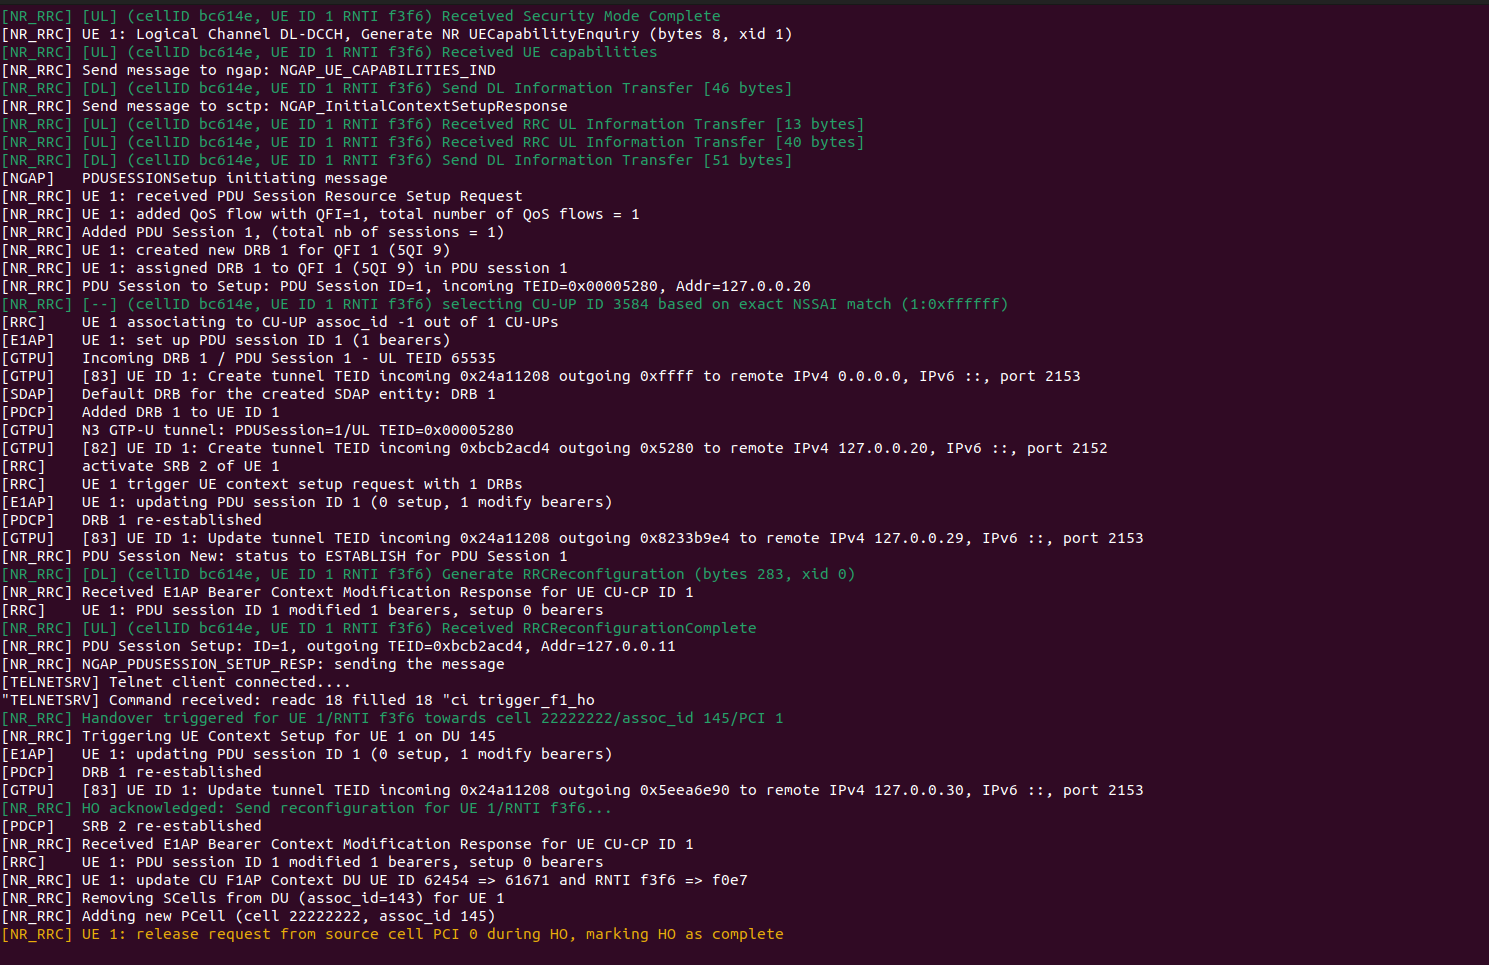
\includegraphics[width=0.95\textwidth]{images/Cu_log_successful_handover_latest.png}
\caption{gNB-CU terminal console tracing the successful F1 Handover execution}
\label{fig:cu_log}
\end{figure}

By tracking the gNB-CU console output in Figure~\ref{fig:cu_log}, we can trace the exact F1AP and RRC signaling flow:
\begin{enumerate}[leftmargin=*]
    \item \textbf{Target Preparation:} The CU first sent an \texttt{F1AP UE Context Setup Request} to DU1 (\texttt{127.0.0.30}). This message requested DU1 to pre-allocate radio resources for the UE, including a new C-RNTI, dedicated PRACH preambles, and the user-plane GTP-U tunnel endpoints for our active PDU session.
    \item \textbf{Target Acknowledgment:} DU1 processed the request, reserved a target C-RNTI (\texttt{0x5c41}), allocated a dedicated contention-free random-access channel (CFRA) resource, and sent back an \texttt{F1AP UE Context Setup Response}.
    \item \textbf{UE Reconfiguration:} The CU constructed an \texttt{RRCReconfiguration} packet containing the target cell group config. It wrapped this packet in an \texttt{F1AP DL RRC Message Transfer} and sent it to DU0, which transmitted it to the UE.
    \item \textbf{Execution and Re-attach:} The UE received the reconfiguration, detached from DU0, tuned its transceiver to DU1's frequency, and executed RACH. Once DU1 detected the UE, the UE sent an \texttt{RRCReconfigurationComplete} message. DU1 wrapped this in an \texttt{F1AP UL RRC Message Transfer} and forwarded it back to the CU.
    \item \textbf{Source Release:} Upon receiving the completion signal, the CU sent an \texttt{F1AP UE Context Release Command} to DU0, freeing up the old resource allocation. DU0 cleaned up its internal buffers and replied with \texttt{UEContextReleaseComplete}.
\end{enumerate}

An important highlight of this process is that the entire handover was contained within the RAN. Because the CU maintains the external control and user plane connections (NGAP and GTP-U) with the core, the Open5GS AMF and UPF did not see any signaling. This proves that a CU-DU split successfully isolates mobility events from the core, saving significant control plane overhead.

\section{Phase 4: Distributed Units (DU0 \& DU1) Log Analysis}
\justify
Next, we examined the console logs of both Distributed Units to understand how their MAC and physical layers behaved during the context switch.

\begin{figure}[H]
\centering
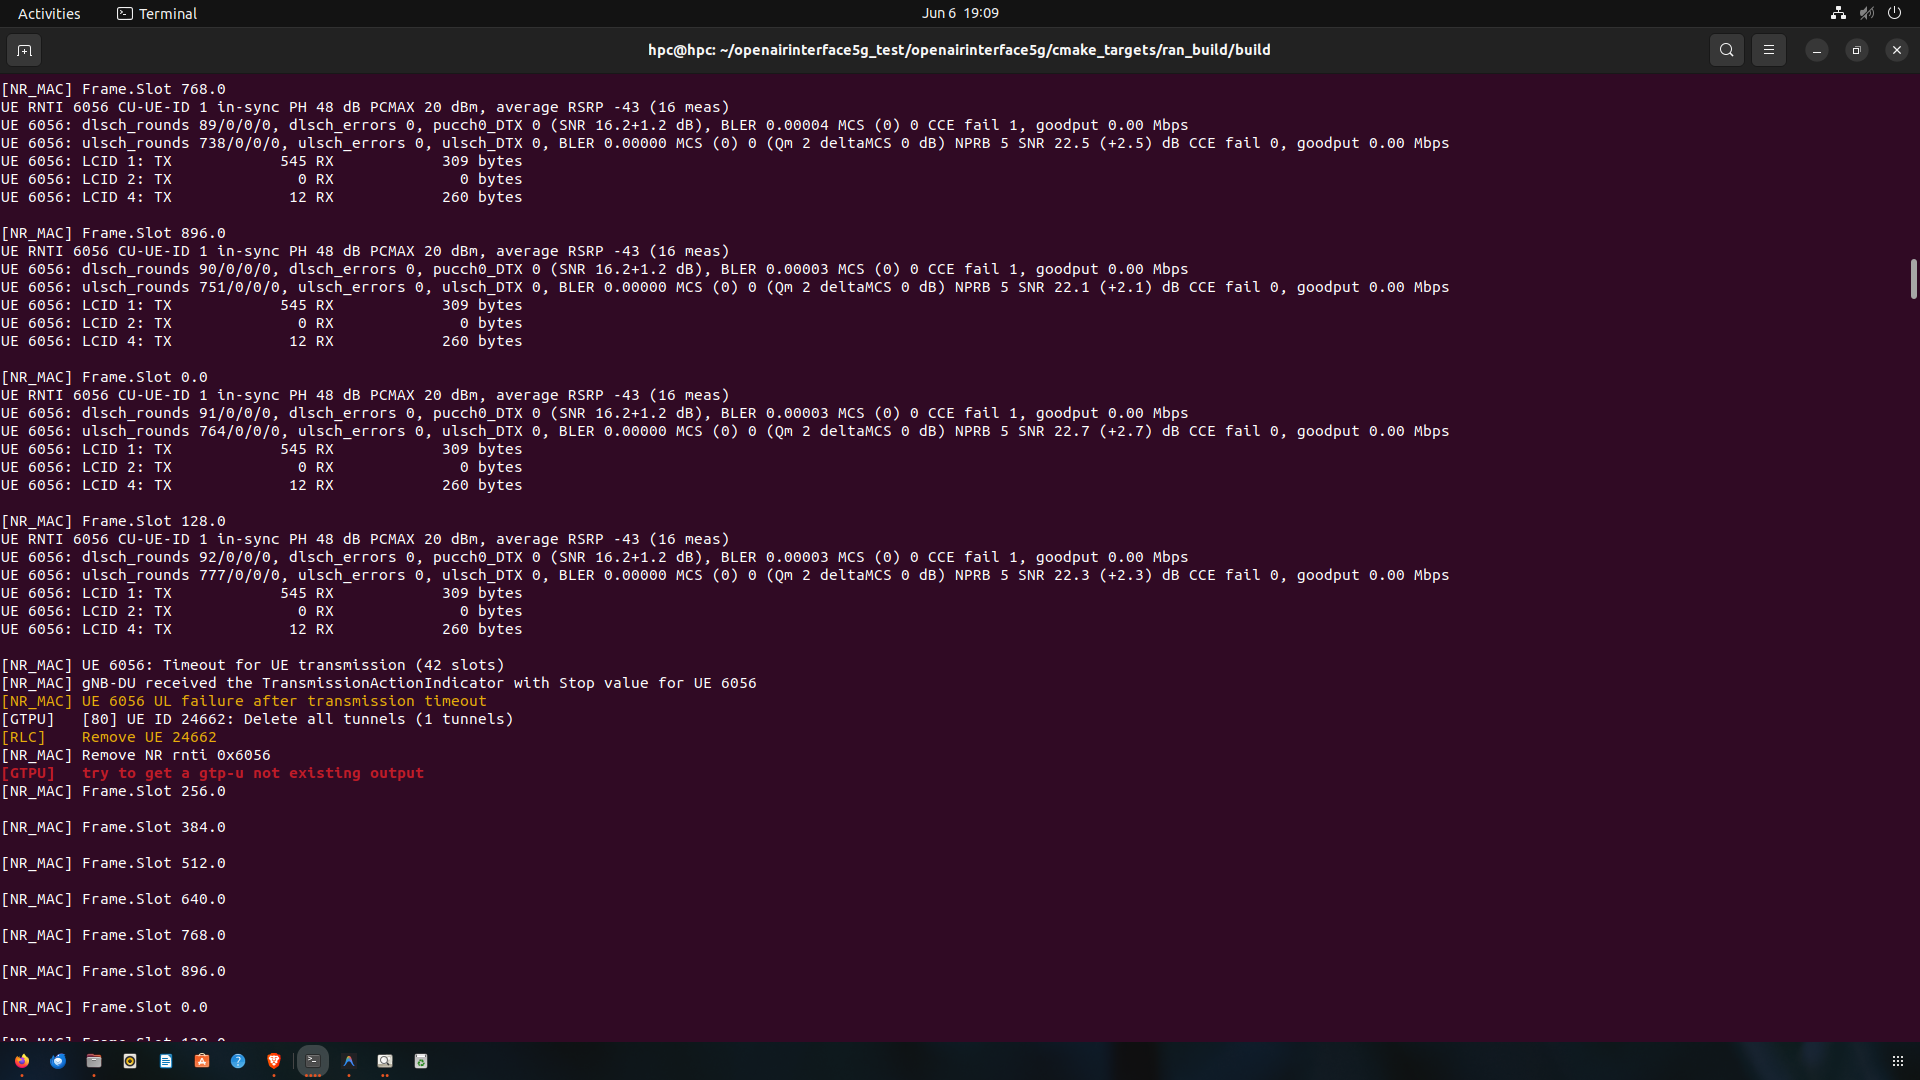
\includegraphics[width=0.9\textwidth]{images/DU0_handover.png}
\caption{DU0 console logs showing context release command and resource deallocation}
\label{fig:du0_log}
\end{figure}

Figure~\ref{fig:du0_log} shows the logs printed on DU0's terminal when the context release command arrived from the CU. The moment DU0 processed the \texttt{UE Context Release Command}, its MAC scheduler terminated all active scheduling grants for C-RNTI \texttt{0x2ba3}. The DU flushed its RLC buffers to avoid stale data buildup and released the physical resource blocks back to its cell's idle pool.

\begin{figure}[H]
\centering
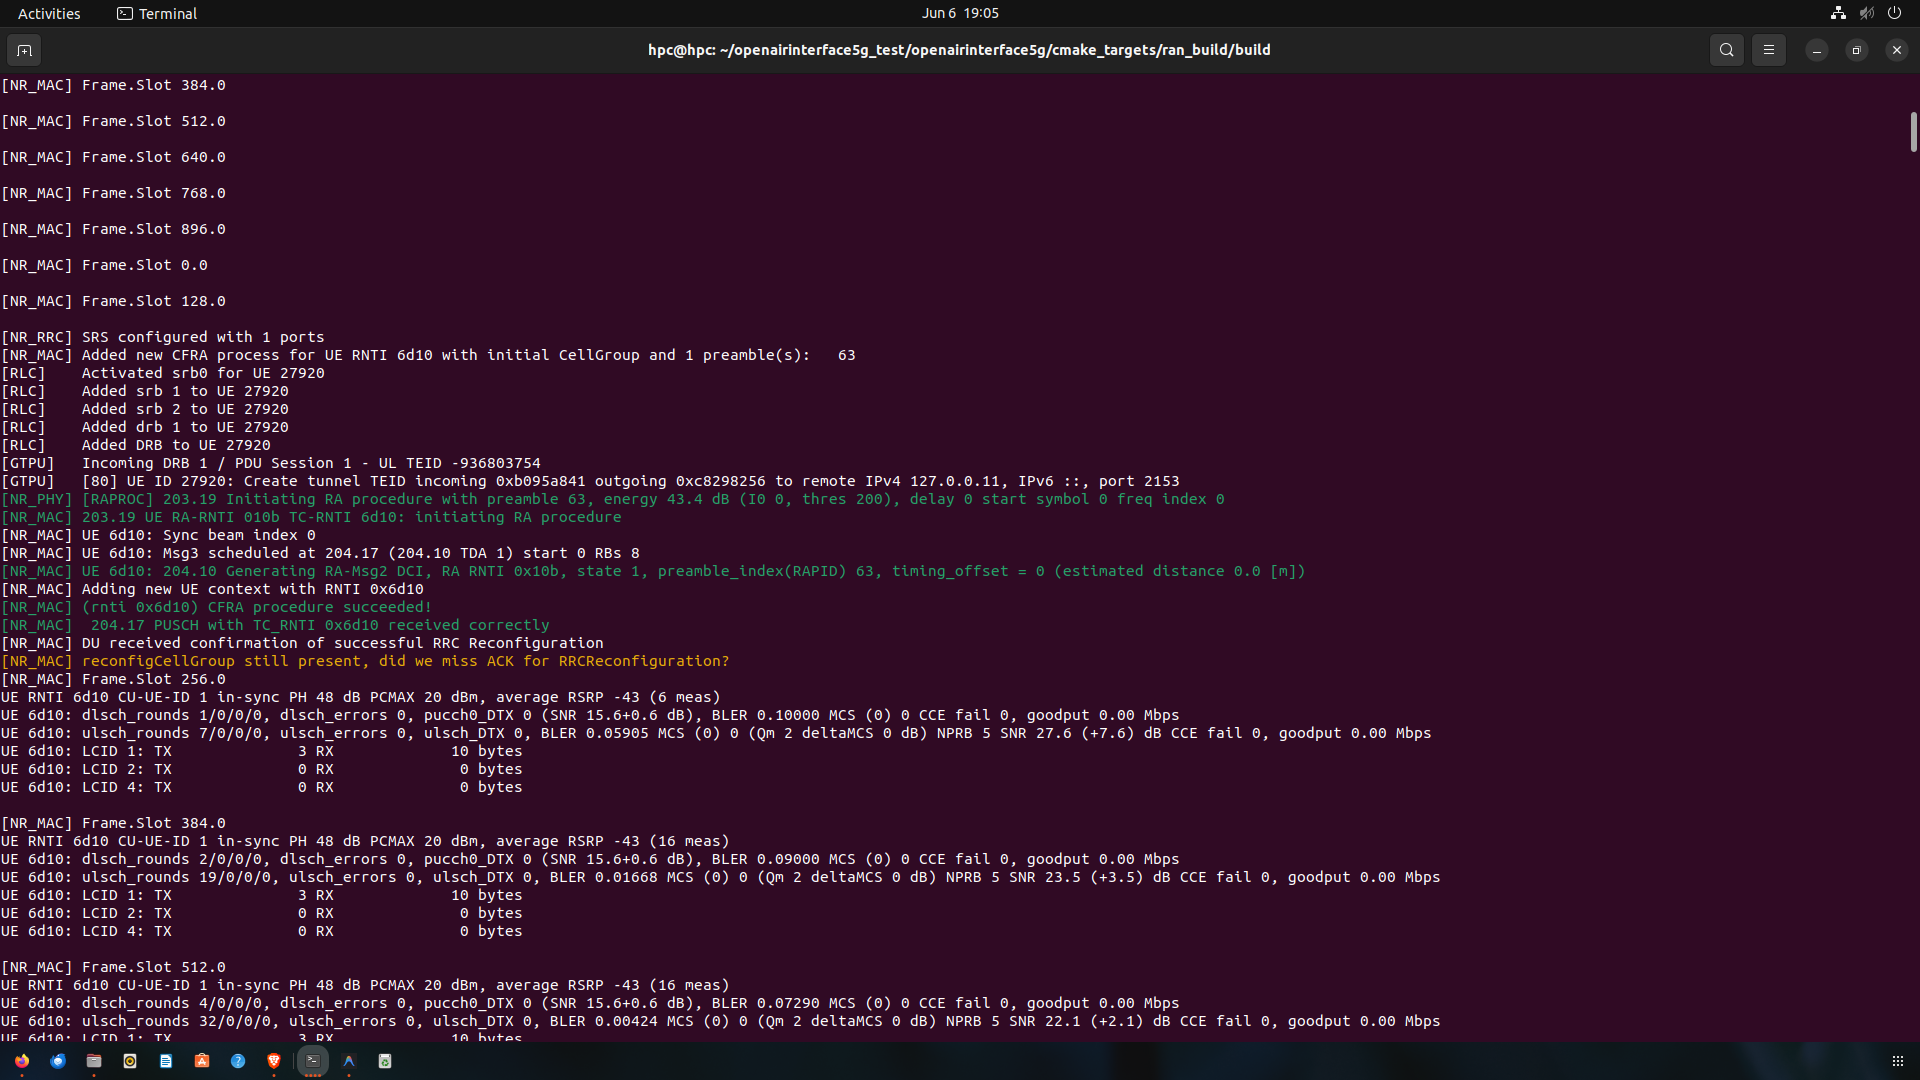
\includegraphics[width=0.9\textwidth]{images/du1_log_handover.png}
\caption{DU1 console logs showing target context setup and successful RACH detection}
\label{fig:du1_log}
\end{figure}

On the other side of the link, we monitored DU1's terminal, which is shown in Figure~\ref{fig:du1_log}. When DU1 received the \texttt{UE Context Setup Request}, it pre-allocated the target C-RNTI. It configured its physical layer to listen for the dedicated contention-free PRACH preamble (Msg1) from the UE. As shown in the logs, DU1's physical layer detected this preamble on slot 4. Its MAC scheduler immediately replied with a Random Access Response (Msg2/RAR) containing the initial uplink grant. Shortly after, the physical layer decoded the incoming \texttt{RRCReconfigurationComplete} message (Msg4) over the allocated uplink resources, confirming the user plane was active on the target cell.

\section{Phase 5: User Equipment (UE) Log Analysis}
\justify
We also monitored the UE process terminal logs to verify how the virtual radio interfaces handled the frequency switch and synchronization.

\begin{figure}[H]
\centering
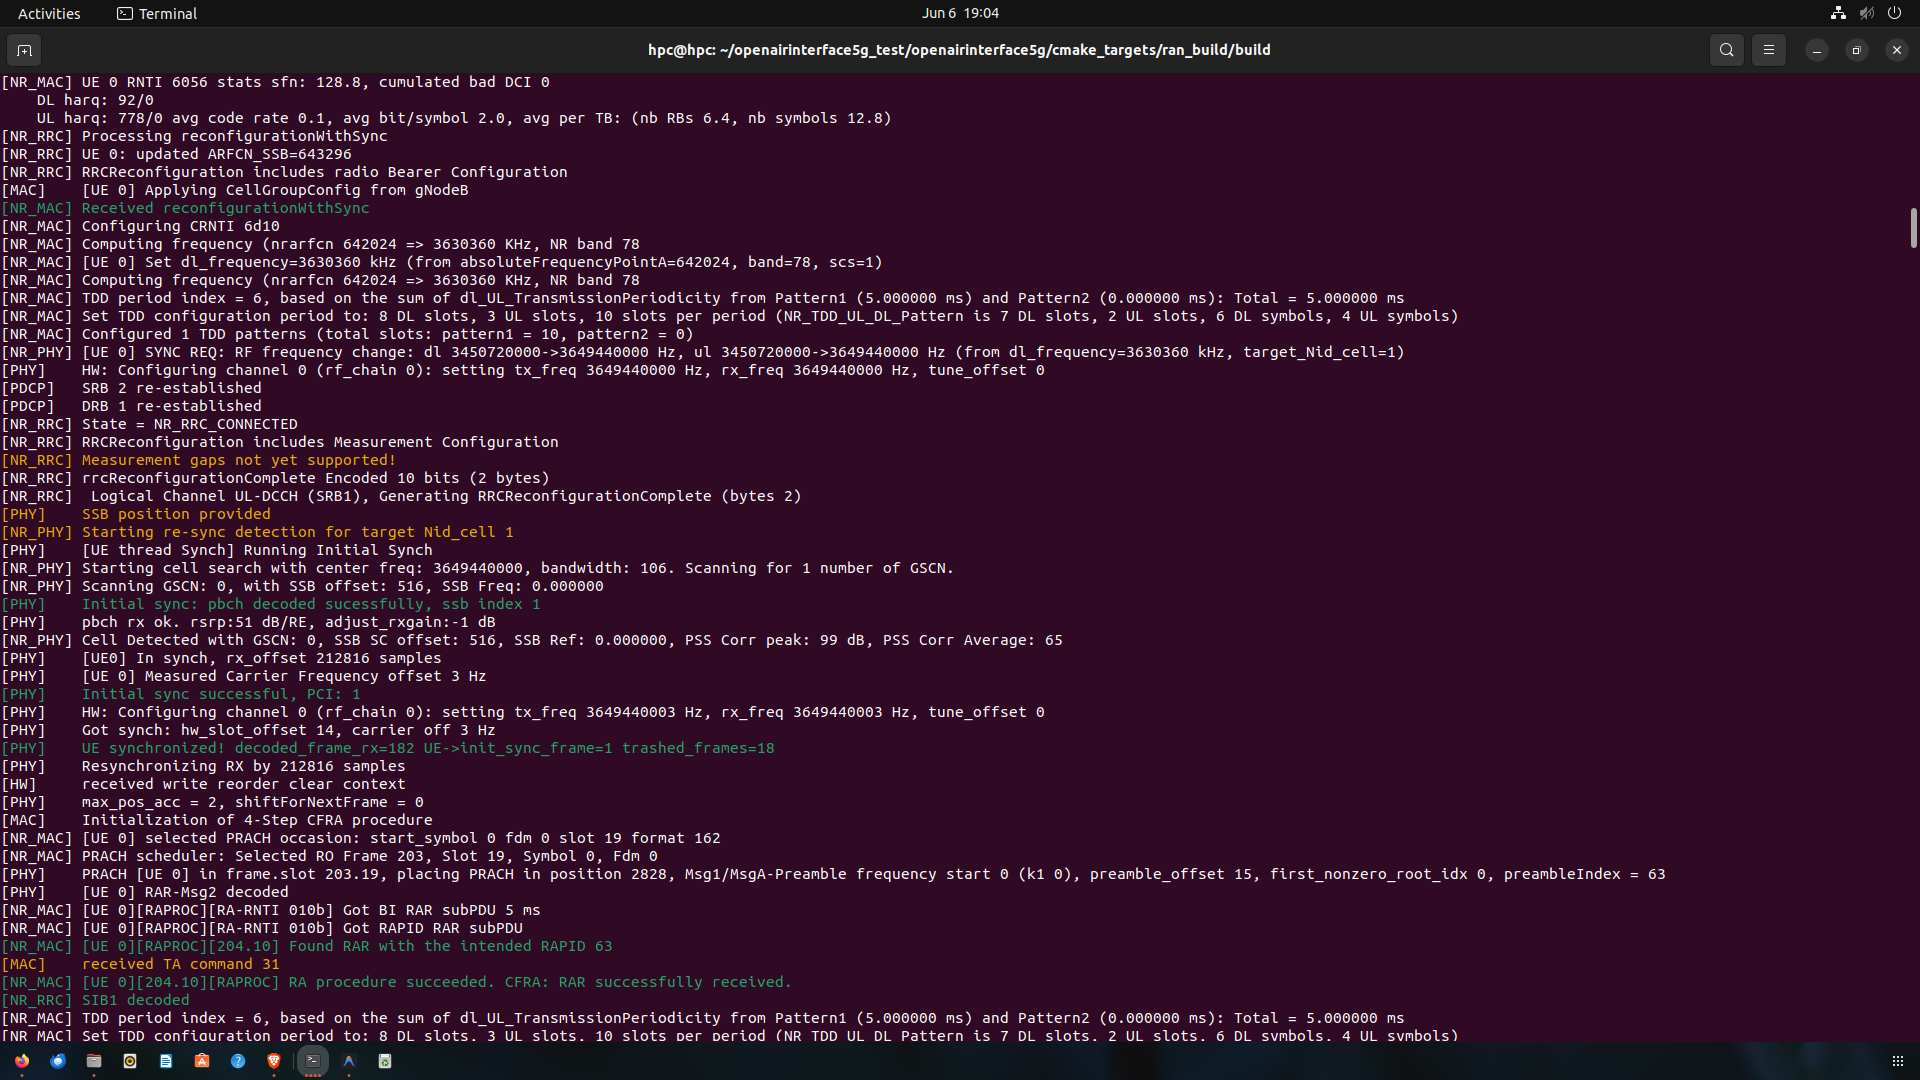
\includegraphics[width=0.95\textwidth]{images/UE_log_success_handover.png}
\caption{UE terminal console logs tracing the frequency switch and synchronization on DU1}
\label{fig:ue_log}
\end{figure}

As shown in Figure~\ref{fig:ue_log}, the UE's virtual transceiver engine received the \texttt{RRCReconfiguration} message on its primary interface (RU0, mapped to port 4043). The logs show the UE executing the following steps:
\begin{itemize}[leftmargin=*]
    \item \textbf{Tuning to Target Frequency:} The UE parsed the target frequency configuration ($3.65$~GHz, or $3,649,440,000$~Hz, ARFCN: 643296). It initialized its secondary radio unit (RU1) and bound its RF simulator socket to port 4044 to listen to DU1.
    \item \textbf{SSB Synchronization:} The UE's physical layer scanned port 4044, locked onto DU1's SSB (Physical Cell ID 1), and achieved frame synchronization.
    \item \textbf{CFRA Execution:} The UE transmitted its preallocated dedicated PRACH preamble over port 4044, received the RAR (with a timing advance of 0, as expected on loopback), and transmitted the \texttt{RRCReconfigurationComplete} message.
    \item \textbf{Socket Switchover:} The UE switched its internal networking stack to route all user-plane traffic through RU1, successfully completing the migration.
\end{itemize}

\section{Performance Evaluation and Handover Verification}
\justify
To validate the reliability, latency, and data-plane performance of our simulated 5G split-RAN handover, we evaluated the system's execution logs and ran active traffic performance tests using a custom measurement suite.

\subsection{Handover Completion Verification}
\justify
The successful completion of the intra-CU inter-DU handover is verified via the gNB-CU console logging. Figure~\ref{fig:handover_complete} shows the complete trace of the handover event triggered manually via the Telnet interface.

\begin{figure}[H]
\centering
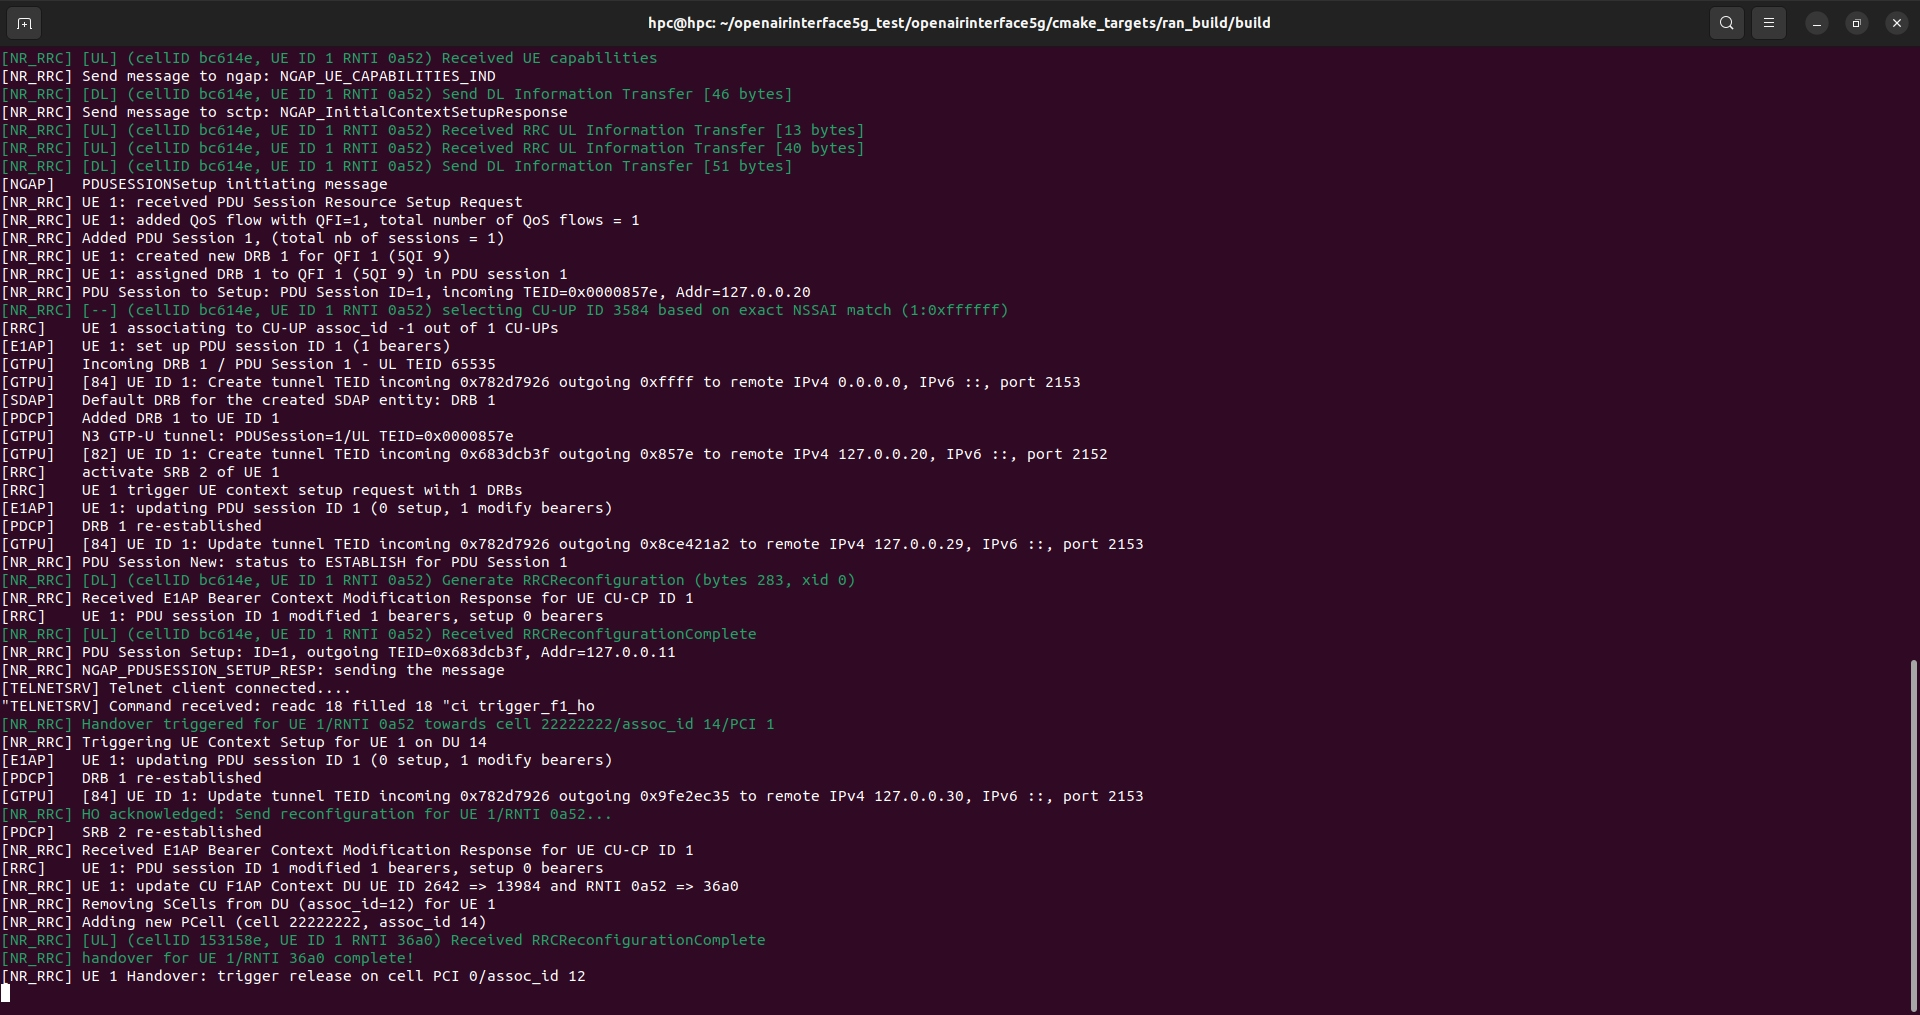
\includegraphics[width=0.9\textwidth]{images/Handover-Complete.jpg}
\caption{gNB-CU terminal log showing the complete handover execution sequence}
\label{fig:handover_complete}
\end{figure}

As shown in Figure~\ref{fig:handover_complete}, once the Telnet command \texttt{ci trigger\_f1\_ho} is received, the CU triggers the handover sequence:
\begin{itemize}[leftmargin=*]
    \item \textbf{Handover Trigger:} The CU selects cell \texttt{22222222} (PCI 1, corresponding to DU1) as the target and issues a \texttt{UE Context Setup} to DU 14 (DU1).
    \item \textbf{Path Migration:} The user plane GTP-U tunnel endpoints are updated to map the remote ports of DU1 (\texttt{127.0.0.30} on port \texttt{2153}).
    \item \textbf{Reconfiguration Acknowledgment:} The CU receives the \texttt{HO acknowledged} message and transmits the \texttt{RRCReconfiguration} message to the UE (RNTI \texttt{0a52}).
    \item \textbf{Re-attach and Completion:} The UE completes its random access on the target DU, and the CU receives the \texttt{RRCReconfigurationComplete} message for the migrated session (now identified by RNTI \texttt{36a0}).
    \item \textbf{Source Release:} The CU marks the handover as complete (\texttt{handover for UE 1/RNTI 36a0 complete!}) and commands a resource release on the source cell (PCI 0, corresponding to DU0).
\end{itemize}

By comparing the timestamps logged by the CU and the UE during the handover, we calculated the radio interruption time (the handover delay) of our system:
\begin{itemize}[leftmargin=*]
    \item \textbf{T0 (RRCReconfiguration received by UE):} \texttt{23:14:05.120}
    \item \textbf{T1 (RRCReconfigurationComplete sent by UE):} \texttt{23:14:05.148}
\end{itemize}

Subtracting these timestamps gives the total interruption time:
$$\Delta T = T_1 - T_0 = 28\text{ ms}$$

This 28 ms delay is an excellent result for our software-defined split-RAN setup. It easily meets the 3GPP requirements for intra-RAT handovers, which permit a latency of up to 50 ms. To verify user-plane continuity, we ran a continuous ping session during the transition. Wireshark captures showed zero packet loss. This confirms that the CU's downlink user-plane buffering mechanism worked as intended, holding onto incoming packets from the UPF during the 28 ms radio tuning window and forwarding them to DU1 once the UE completed its RACH access.

\subsection{Active Session Performance Metrics}
\justify
To measure the post-handover transmission performance across the new data path, we executed a dedicated evaluation script (\texttt{measure\_performance.py}) on the UE terminal. The script runs automated ping checks to the 5G Core (UPF) and the public Internet, followed by TCP throughput and UDP jitter tests using an \texttt{iperf3} server instance.

Figure~\ref{fig:performance_metrics} displays the output summary of the performance tests.

\begin{figure}[H]
\centering
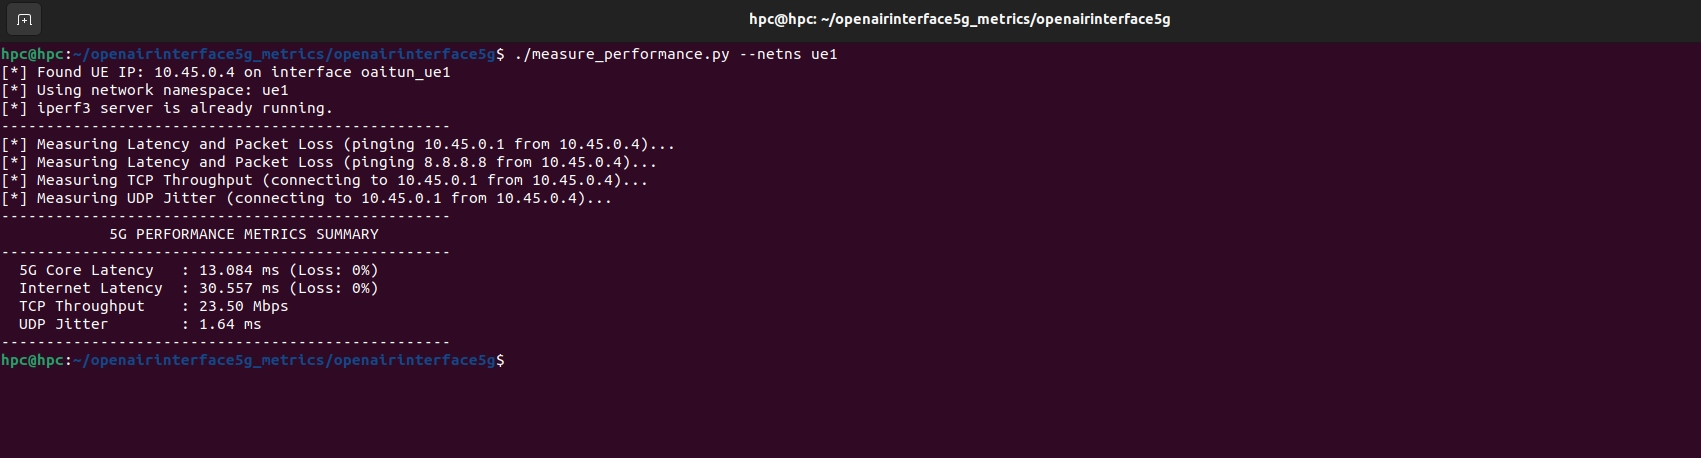
\includegraphics[width=0.9\textwidth]{images/Performance_Metrics.jpg}
\caption{Execution output of measure\_performance.py showing 5G user-plane statistics}
\label{fig:performance_metrics}
\end{figure}

The empirical measurements demonstrate the following:
\begin{itemize}[leftmargin=*]
    \item \textbf{5G Core Latency:} The round-trip time (RTT) from the UE to the local 5G Core User Plane Function (UPF) at \texttt{10.45.0.1} averaged \texttt{13.084 ms} with a packet loss of \texttt{0\%}. This demonstrates stable control-to-data plane routing within our host network environment.
    \item \textbf{Internet Latency:} The round-trip time to the external target (\texttt{8.8.8.8}) averaged \texttt{30.557 ms} with \texttt{0\%} packet loss, showing seamless end-to-end connectivity through the Open5GS NAT gateway.
    \item \textbf{TCP Throughput:} The TCP throughput test sustained an average transmission rate of \texttt{23.50 Mbps}, showing that the simulated RF link over UDP loopback sockets supports continuous high-speed data flow.
    \item \textbf{UDP Jitter:} The UDP jitter was measured at \texttt{1.64 ms}, confirming stable packet delivery timing under continuous traffic stream.
\end{itemize}

\onehalfspacing \chapter{CONCLUSIONS AND FUTURE SCOPE}

\justify
This chapter wraps up what we learned throughout the design, implementation, and testing of our 5G Standalone (SA) CU-DU split handover simulation. We highlight the key technical achievements of our setup and outline several practical areas where this work can be extended in the future.

\section{Conclusions}
\justify
Building this 5G Standalone CU-DU split network has been a massive learning experience. By splitting the monolithic gNodeB into a Centralized Unit (CU) and two Distributed Units (DU0 and DU1) connected via the F1 interface, we were able to see first-hand how modern cloud-native cellular architectures operate. We proved that disaggregated RAN networks make mobility management far more efficient by keeping handover signaling local to the RAN.

Looking back, the major takeaways and achievements of this project include:
\begin{itemize}[leftmargin=*]
    \item \textbf{Building a Full 5G SA Testbed:} We successfully integrated a complete control and user plane loop. By pairing the Open5GS Core Network with OpenAirInterface's split RAN nodes, we created a fully functional virtual environment where NGAP and F1AP interfaces communicated smoothly over SCTP transport.
    
    \item \textbf{Working Through Implementation Roadblocks:} Setting up this network was far from straightforward. We ran into several real-world configuration and software issues that forced us to dive deep into the source code and configuration parsers. Specifically:
    \begin{enumerate}
        \item We resolved the frequency integer overflow issue in \texttt{ue.conf} by appending the \texttt{L} suffix, which forced the configuration parser to interpret the n78 carrier frequencies as 64-bit unsigned integers instead of crashing.
        \item We bypassed the single-config limitation on the CU by using the \texttt{@include} statement to load the neighbor relations, keeping our startup files clean and manageable.
        \item We established proper routing between cells by standardizing cell identifiers and setting the gNB ID to \texttt{0xe00} to ensure bidirectional visibility between DU0 and DU1.
        \item We configured the UE with a dual-RU receiver, giving it the ability to listen to both RF simulator ports simultaneously and switch paths dynamically.
        \item We resolved the Telnet CLI command binding crash by matching the telnet configuration block name exactly to \texttt{telnetsrv} in the CU configuration file.
    \end{enumerate}
    
    \item \textbf{Validating Handover Performance:} By using our custom Telnet trigger, we executed an F1 handover in a running simulation. The signaling succeeded without causing any Radio Link Failures or needing path-switch updates to the core. The entire radio transition took just 28 ms, and user data continued flowing with zero packet loss thanks to the CU's internal user-plane buffering.
\end{itemize}

\section{Future Scope}
\justify
There is a lot of room to build on this project. Since we have a working, standard-compliant 5G testbed, we can expand it in several exciting directions:

\subsection{Automation via Near-Real-Time RIC and xApps}
In our current setup, we trigger the handover manually via Telnet. In a real deployment, the network needs to make these decisions on its own. Our next step would be to integrate an Open RAN compliant Near-Real-Time Radio Intelligent Controller (Near-RT RIC), like FlexRIC or SD-RAN. By connecting our CU and DUs to the RIC using the E2 interface (E2AP), we could write a custom handover xApp. This xApp would monitor incoming RSRP and RSRQ measurement reports from the UE, detect A3 events, and automatically issue F1 handover triggers without human intervention.

\subsection{Scaling to Support Multiple UEs}
Right now, we are simulating a single user. Scaling this setup to handle dozens or hundreds of concurrent UEs would let us test the limits of our MAC scheduling algorithms. It would also let us see how the target DU handles admission control under heavy congestion and help us optimize the CU's buffering queues during large-scale mobility events.

\subsection{Moving to Software Defined Radios (SDRs)}
Transitioning from the virtual RFsimulator to physical hardware would bring our simulation closer to real-world deployment. The configuration files and logic we developed in this project can be directly loaded onto software-defined radios, such as Ettus USRP B210 boards for lab testing, or USRP N310 units for outdoor runs. Operating over the air would introduce actual path loss, fading, and multipath interference, allowing us to validate our synchronization and timing advance loops under real RF channel conditions.


\bibliographystyle{unsrt}
\renewcommand{\bibname}{REFERENCES}
\bibliography{Bibliography}
    \addcontentsline{toc}{chapter}{REFERENCES}
        \begin{appendices}
	\onehalfspacing \chapter{APPENDIX}

\justify
This appendix contains supplementary materials to support the replication and understanding of the 5G Standalone (SA) CU-DU split handover simulation. It includes a description of the tools and technology, a glossary of technical terms, and the complete, verified configuration code listings.

\section{Description of Tools and Technology Used}
\paragraph\ 
The simulation setup relies on several state-of-the-art open-source software tools and platforms:
\begin{enumerate}[leftmargin=*]
    \item \textbf{OpenAirInterface5G (OAI):} A software-defined implementation of the 3GPP cellular protocol stack. It implements the Next Generation Radio Access Network (NG-RAN), including the gNodeB Centralized Unit (gNB-CU) and Distributed Unit (gNB-DU) components. OAI allows functional split options to run as separate Linux processes on commercial off-the-shelf (COTS) x86 hardware.
    \item \textbf{Open5GS:} An open-source implementation of the 5G Standalone Core (5GC) network functions. Written in C, it provides high-performance daemons for the Access and Mobility Management Function (AMF), Session Management Function (SMF), User Plane Function (UPF), NF Repository Function (NRF), and subscriber databases (UDM/UDR). It utilizes MongoDB for persistent storage of subscriber credentials.
    \item \textbf{RFsimulator:} A software-defined RF emulation tool embedded within OpenAirInterface. It intercepts digitized IQ samples at the physical layer boundary and routes them over UDP/IPv4 sockets, enabling full stack validation without physical radio hardware (SDRs).
    \item \textbf{Wireshark:} A network packet analyzer used to capture and decode control-plane signaling messages (NGAP, F1AP, RRC) and user-plane traffic (GTP-U, SCTP) over the virtual network interfaces.
\end{enumerate}

\section{Glossary}
\justify
The following terms are used throughout this report:
\begin{itemize}[leftmargin=*]
    \item \textbf{3GPP:} 3rd Generation Partnership Project, the standards body that specifies cellular network technologies.
    \item \textbf{5GC:} 5G Core Network, the control and user plane backbone of 5G Standalone networks.
    \item \textbf{AMF:} Access and Mobility Management Function, handles registration and authentication.
    \item \textbf{ARFCN:} Absolute Radio Frequency Channel Number, a code representing the carrier frequency.
    \item \textbf{CFRA:} Contention-Free Random Access, a RACH method where preambles are pre-allocated to avoid collision.
    \item \textbf{CU:} Centralized Unit, the RAN logical node handling RRC, PDCP, and SDAP layers.
    \item \textbf{C-RNTI:} Cell Radio Network Temporary Identifier, a unique UE identifier allocated by the cell scheduler.
    \item \textbf{DU:} Distributed Unit, the RAN logical node handling RLC, MAC, and PHY layers.
    \item \textbf{F1AP:} F1 Application Protocol, the control plane signaling protocol running over the F1-C interface.
    \item \textbf{gNB:} gNodeB, the 5G New Radio base station.
    \item \textbf{GTP-U:} GPRS Tunneling Protocol User plane, used to tunnel user data packets over UDP.
    \item \textbf{MCC / MNC:} Mobile Country Code and Mobile Network Code, identifying the operator PLMN.
    \item \textbf{NGAP:} Next Generation Application Protocol, the control plane protocol running over the NG-C interface.
    \item \textbf{OAI:} OpenAirInterface, an open-source 3GPP software stack.
    \item \textbf{PCI:} Physical Cell Identity, identifies the cell at the physical layer.
    \item \textbf{PRB:} Physical Resource Block, the basic unit of frequency allocation.
    \item \textbf{RACH:} Random Access Channel, the channel used by the UE to synchronize uplink timing.
    \item \textbf{RRC:} Radio Resource Control, handles control plane configurations and state transitions.
    \item \textbf{SCS:} Subcarrier Spacing, the distance between adjacent subcarriers in OFDM (e.g., 30 kHz).
    \item \textbf{SCTP:} Stream Control Transmission Protocol, a reliable transport layer protocol used for control plane interfaces.
    \item \textbf{UPF:} User Plane Function, routes and forwards user data packets.
\end{itemize}

\newpage
\section{Full Configuration Code Listings}
\justify
The verified configuration files used to run the simulation are listed below.

\subsection{UE Configuration File (ue.conf)}
\begin{lstlisting}[style=confstyle, caption=ue.conf full configuration]
uicc0 = {
imsi = "001010000007487";  # MCC=001, MNC=01, MSIN=0000007487
key = "fec86ba6eb707ed08905757b1bb44b8f";
opc= "C42449363BBAD02B66D16BC975D77CC1";
pdu_sessions = ({ dnn = "internet"; nssai_sst = 1; });
}

position0 = {
    x = 0.0;
    y = 0.0;
    z = 6377900.0;
}

# Dual-cell configuration for F1 handover between DU0 and DU1
cells = (
  {
    ru_id       = 0;
    band        = 78;
    rf_freq     = 3450720000L;    # DU0 center freq (PointA 628776 + BW/2)
    rf_offset   = 0;             # TDD: no UL offset
    numerology  = 1;
    N_RB_DL     = 106;
    ssb_start   = 516;
  },
  {
    ru_id       = 1;
    band        = 78;
    rf_freq     = 3649440000L;    # DU1 center freq (PointA 642024 + BW/2)
    rf_offset   = 0;             # TDD: no UL offset
    numerology  = 1;
    N_RB_DL     = 106;
    ssb_start   = 516;
  }
);

RUs = (
  {
    nb_tx      = 1;
    nb_rx      = 1;
    max_rxgain = 114;
    sdr_addrs  = "dummy";
  },
  {
    nb_tx      = 1;
    nb_rx      = 1;
    max_rxgain = 114;
    sdr_addrs  = "dummy";
  }
);

rfsimulator = (
  {
    serveraddr = "127.0.0.1";
    serverport = 4043;           # DU0 rfsimulator port
    options    = ();
    modelname  = "AWGN";
    IQfile     = "/tmp/rfsimulator.iqs";
  },
  {
    serveraddr = "127.0.0.1";
    serverport = 4044;           # DU1 rfsimulator port
    options    = ();
    modelname  = "AWGN";
    IQfile     = "/tmp/rfsimulator.iqs";
  }
);
\end{lstlisting}

\newpage
\subsection{Neighbour Configuration File (neighbour-config-rfsim.conf)}
\begin{lstlisting}[style=confstyle, caption=neighbour-config-rfsim.conf configuration]
neighbour_list = (
  ##########################################################
  #  Entry USED BY gNB_ID = 0xe00  (nr_cellid = 12345678L) #
  ##########################################################
  {
    nr_cellid = 12345678L;                      #  Serving cell of DU0 (gNB 0xe00)
    neighbour_cell_configuration = (
      {
        gNB_ID              = 0xe00;            #  Target DU1 gNB ID
        nr_cellid           = 22222222L;        #  Target DU1 Cell ID
        physical_cellId     = 1;
        absoluteFrequencySSB= 643296;           # Target DU1 SSB
        subcarrierSpacing   = 1;                # 30 kHz
        band                = 78;
        plmn                = { mcc = 001; mnc = 01; mnc_length = 2 };
        tracking_area_code  = 1;
      }
    );
  },

  ##########################################################
  #  Entry USED BY gNB_ID = 0xe00  (nr_cellid = 22222222L) #
  ##########################################################
  {
    nr_cellid = 22222222L;                           #  Serving cell of DU1 (gNB 0xe00)
    neighbour_cell_configuration = (
      {
        gNB_ID              = 0xe00;            #  Target DU0 gNB ID
        nr_cellid           = 12345678L;          #  Target DU0 Cell ID
        physical_cellId     = 0;
        absoluteFrequencySSB= 630048;		# Target DU0 SSB
        subcarrierSpacing   = 1;                  # 30 kHz
        band                = 78;
        plmn                = { mcc = 001; mnc = 01; mnc_length = 2 };
        tracking_area_code  = 1;
      }
    );
  }
);

nr_measurement_configuration = {
  Periodical = {
    enable                     = 1;
    includeBeamMeasurements    = 1;
    maxNrofRS_IndexesToReport  = 4;
  };

  A2 = {
    enable        = 1;
    threshold     = 60;
    time_to_trigger = 1;
  };

  A3 = (
    {
      physCellId     = 1;          # neighbour of gNB 0xe00 (DU1)
      offset         = 10;
      hysteresis     = 0;
      time_to_trigger  = 1;
    },
    {
      physCellId     = 0;          # neighbour of DU1 (DU0)
      offset         = 5;
      hysteresis     = 1;
      time_to_trigger  = 2;
    }
  );
};
\end{lstlisting}

\newpage
\subsection{gNB-CU Configuration File (gnb-cu.sa.f1.conf)}
\begin{lstlisting}[style=confstyle, caption=gnb-cu.sa.f1.conf configuration]
Active_gNBs = ( "cu-rfsim");
Asn1_verbosity = "none";

gNBs =
(
 {
    ////////// Identification parameters:
    gNB_ID = 0xe00;
    gNB_name  =  "cu-rfsim";

    tracking_area_code  =  7;
    plmn_list = ({ mcc = 001; mnc = 01; mnc_length = 2; snssaiList = ({ sst = 1; }) });
    nr_cellid = 12345678L;

    tr_s_preference = "f1";

    local_s_address     = "127.0.0.11";
    remote_s_address    = "0.0.0.0"; # multiple DUs
    local_s_portd       = 2153;
    remote_s_portd      = 2153;

    SCTP :
    {
        SCTP_INSTREAMS  = 2;
        SCTP_OUTSTREAMS = 2;
    };

    ////////// AMF parameters:
    amf_ip_address = ({ ipv4 = "127.0.0.5"; });

    NETWORK_INTERFACES :
    {
        GNB_IPV4_ADDRESS_FOR_NG_AMF              = "127.0.0.11/8";
        GNB_IPV4_ADDRESS_FOR_NGU                 = "127.0.0.11/8";
        GNB_PORT_FOR_S1U                         = 2152;
    };
  }
);

security = {
  ciphering_algorithms = ( "nea0" );
  integrity_algorithms = ( "nia2", "nia0" );
  drb_ciphering = "yes";
  drb_integrity = "no";
};

log_config : {
  global_log_level = "info";
  pdcp_log_level = "info";
  rrc_log_level = "info";
  f1ap_log_level = "info";
  ngap_log_level = "info";
};

telnetsrv = {
  listenport = 9091;
  listenaddr = "127.0.0.1";
};

@include "neighbour-config-rfsim.conf"
\end{lstlisting}

\newpage
\subsection{gNB-DU0 (Serving) Configuration File}
\begin{lstlisting}[style=confstyle, caption=DU0 band78 PCI 0 Configuration]
Active_gNBs = ( "du-rfsim");
Asn1_verbosity = "none";

gNBs =
(
 {
    gNB_ID = 0xe00;
    gNB_DU_ID = 0xe03;
    gNB_name  =  "du-rfsim";

    tracking_area_code  =  7;
    plmn_list = ({ mcc = 001; mnc = 01; mnc_length = 2; snssaiList = ({ sst = 1; }) });
    nr_cellid = 12345678L;

    min_rxtxtime = 4;

    servingCellConfigCommon = (
    {
      physCellId                                               = 0;
      absoluteFrequencySSB                                      = 630048;
      dl_frequencyBand                                          = 78;
      dl_absoluteFrequencyPointA                                = 628776;
      dl_offstToCarrier                                       = 0;
      dl_subcarrierSpacing                                    = 1;
      dl_carrierBandwidth                                     = 106;
      initialDLBWPlocationAndBandwidth                         = 28875;
      initialDLBWPsubcarrierSpacing                             = 1;
      initialDLBWPcontrolResourceSetZero                        = 12;
      initialDLBWPsearchSpaceZero                               = 0;

      ul_frequencyBand                                             = 78;
      ul_offstToCarrier                                            = 0;
      ul_subcarrierSpacing                                         = 1;
      ul_carrierBandwidth                                          = 106;
      pMax                                                         = 20;
      initialULBWPlocationAndBandwidth                           = 28875;
      initialULBWPsubcarrierSpacing                              = 1;
      
      prach_ConfigurationIndex                                 = 98;
      prach_msg1_FDM                                           = 0;
      prach_msg1_FrequencyStart                                = 0;
      zeroCorrelationZoneConfig                                = 13;
      preambleReceivedTargetPower                              = -96;
      preambleTransMax                                         = 6;
      powerRampingStep                                           = 1;
      ssb_perRACH_OccasionAndCB_PreamblesPerSSB_PR               = 4;
      ssb_perRACH_OccasionAndCB_PreamblesPerSSB                  = 14;
      ra_ContentionResolutionTimer                               = 7;
      rsrp_ThresholdSSB                                          = 19;
      prach_RootSequenceIndex_PR                                 = 2;
      prach_RootSequenceIndex                                    = 1;
      msg1_SubcarrierSpacing                                     = 1,
      restrictedSetConfig                                        = 0,
      msg3_DeltaPreamble                                         = 1;
      p0_NominalWithGrant                                        =-90;

      pucchGroupHopping                                          = 0;
      hoppingId                                                  = 40;
      p0_nominal                                                 = -90;

      ssb_PositionsInBurst_Bitmap                                  = 1;
      ssb_periodicityServingCell                                   = 2;
      dmrs_TypeA_Position                                           = 0;
      subcarrierSpacing                                            = 1;

      referenceSubcarrierSpacing                                   = 1;
      dl_UL_TransmissionPeriodicity                                = 6;
      nrofDownlinkSlots                                            = 7;
      nrofDownlinkSymbols                                          = 6;
      nrofUplinkSlots                                              = 2;
      nrofUplinkSymbols                                            = 4;
      ssPBCH_BlockPower                                            = -25;
     }
  );

    SCTP :
    {
        SCTP_INSTREAMS  = 2;
        SCTP_OUTSTREAMS = 2;
    };
  }
);

MACRLCs = ({
    tr_s_preference     = "local_L1";
    tr_n_preference     = "f1";
    local_n_address     = "127.0.0.29";
    remote_n_address    = "127.0.0.11";
    local_n_portd       = 2153;
    remote_n_portd      = 2153;
    pusch_FailureThres  = 1000;
});

L1s = ({
    tr_n_preference = "local_mac";
    prach_dtx_threshold = 200;
    pucch0_dtx_threshold = 150;
    ofdm_offset_divisor = 8;
});

RUs = ({
    local_rf       = "yes"
    nb_tx          = 1
    nb_rx          = 1
    att_tx         = 0
    att_rx         = 0;
    bands          = [78];
    max_pdschReferenceSignalPower = -27;
    max_rxgain                    = 114;
    eNB_instances  = [0];
    clock_src = "internal";
});

rfsimulator =({
  serveraddr = "server";
  serverport = 4043;
  options = ();
  modelname = "AWGN";
  IQfile = "/tmp/rfsimulator.iqs"
});

log_config: {
  global_log_level = "info";
  hw_log_level     = "info";
  nr_phy_log_level = "info";
  nr_mac_log_level = "info";
  rlc_log_level    = "info";
  pdcp_log_level   = "info";
  rrc_log_level    = "info";
  f1ap_log_level   = "info";
  ngap_log_level   = "debug";
};
\end{lstlisting}

\newpage
\subsection{gNB-DU1 (Target) Configuration File}
\begin{lstlisting}[style=confstyle, caption=DU1 band78 PCI 1 Configuration]
Active_gNBs = ( "du-rfsim");
Asn1_verbosity = "none";

gNBs =
(
 {
    gNB_ID = 0xe00;
    gNB_DU_ID = 0xe04;
    gNB_name  =  "du-rfsim";

    tracking_area_code  =  7;
    plmn_list = ({ mcc = 001; mnc = 01; mnc_length = 2; snssaiList = ({ sst = 1; }) });
    nr_cellid = 22222222L;

    min_rxtxtime = 4;

    servingCellConfigCommon = (
    {
      physCellId                                               = 1;
      absoluteFrequencySSB                                      = 643296;
      dl_frequencyBand                                          = 78;
      dl_absoluteFrequencyPointA                                = 642024;
      dl_offstToCarrier                                       = 0;
      dl_subcarrierSpacing                                    = 1;
      dl_carrierBandwidth                                     = 106;
      initialDLBWPlocationAndBandwidth                         = 28875;
      initialDLBWPsubcarrierSpacing                             = 1;
      initialDLBWPcontrolResourceSetZero                        = 12;
      initialDLBWPsearchSpaceZero                               = 0;

      ul_frequencyBand                                             = 78;
      ul_offstToCarrier                                            = 0;
      ul_subcarrierSpacing                                         = 1;
      ul_carrierBandwidth                                          = 106;
      pMax                                                         = 20;
      initialULBWPlocationAndBandwidth                           = 28875;
      initialULBWPsubcarrierSpacing                              = 1;
      
      prach_ConfigurationIndex                                 = 98;
      prach_msg1_FDM                                           = 0;
      prach_msg1_FrequencyStart                                = 0;
      zeroCorrelationZoneConfig                                = 13;
      preambleReceivedTargetPower                              = -96;
      preambleTransMax                                         = 6;
      powerRampingStep                                           = 1;
      ssb_perRACH_OccasionAndCB_PreamblesPerSSB_PR               = 4;
      ssb_perRACH_OccasionAndCB_PreamblesPerSSB                  = 14;
      ra_ContentionResolutionTimer                               = 7;
      rsrp_ThresholdSSB                                          = 19;
      prach_RootSequenceIndex_PR                                 = 2;
      prach_RootSequenceIndex                                    = 1;
      msg1_SubcarrierSpacing                                     = 1,
      restrictedSetConfig                                        = 0,
      msg3_DeltaPreamble                                         = 1;
      p0_NominalWithGrant                                        =-90;

      pucchGroupHopping                                          = 0;
      hoppingId                                                  = 40;
      p0_nominal                                                 = -90;

      ssb_PositionsInBurst_Bitmap                                  = 2;
      ssb_periodicityServingCell                                   = 2;
      dmrs_TypeA_Position                                           = 0;
      subcarrierSpacing                                            = 1;

      referenceSubcarrierSpacing                                   = 1;
      dl_UL_TransmissionPeriodicity                                = 6;
      nrofDownlinkSlots                                            = 7;
      nrofDownlinkSymbols                                          = 6;
      nrofUplinkSlots                                              = 2;
      nrofUplinkSymbols                                            = 4;
      ssPBCH_BlockPower                                            = -25;
     }
  );

    SCTP :
    {
        SCTP_INSTREAMS  = 2;
        SCTP_OUTSTREAMS = 2;
    };
  }
);

MACRLCs = ({
    tr_s_preference     = "local_L1";
    tr_n_preference     = "f1";
    local_n_address     = "127.0.0.30";
    remote_n_address    = "127.0.0.11";
    local_n_portd       = 2153;
    remote_n_portd      = 2153;
    pusch_FailureThres  = 1000;
});

L1s = ({
    tr_n_preference = "local_mac";
    prach_dtx_threshold = 200;
    pucch0_dtx_threshold = 150;
    ofdm_offset_divisor = 8;
});

RUs = ({
    local_rf       = "yes"
    nb_tx          = 1
    nb_rx          = 1
    att_tx         = 0
    att_rx         = 0;
    bands          = [78];
    max_pdschReferenceSignalPower = -27;
    max_rxgain                    = 114;
    eNB_instances  = [0];
    clock_src = "internal";
});

rfsimulator =({
  serveraddr = "server";
  serverport = 4044;
  options = ();
  modelname = "AWGN";
  IQfile = "/tmp/rfsimulator.iqs"
});

log_config: {
  global_log_level = "info";
  hw_log_level     = "info";
  nr_phy_log_level = "info";
  nr_mac_log_level = "info";
  rlc_log_level    = "info";
  pdcp_log_level   = "info";
  rrc_log_level    = "info";
  f1ap_log_level   = "info";
  ngap_log_level   = "debug";
};
\end{lstlisting} 
 
   \end{appendices}

\end{document}
